%% Преамбула TeX-файла

% 1. Стиль и язык
\documentclass[utf8x, 14pt]{G7-32} % Стиль (по умолчанию будет 14pt)

% Остальные стандартные настройки убраны в preamble.inc.tex.
%\Referat

Расчетно-пояснительная записка содержит \pageref{LastPage} страницы, 66 рисунков, 21 таблицу, 46 источников, 6 приложений.

Ключевые слова: противотанковая управляемая ракета, беспилотный авиационный комплекс, разведывательно-ударный беспилотный летательный аппарат, моделирование траектории полета, твердотопливный ускоритель.

Цель выпускной квалификационной работы – проектирование противотанкового комплекса на базе разведывательного-ударного БПЛА и проработка оценки эффективности применения противотанковой управляемой ракеты (ПТУР), входящей в состав комплекса.

Решаемые задачи:
\begin{itemize}
	\item Формирование облика и структуры комплекса;
	\item Проектирование противотанковой управляемой ракеты;
	\item Разработка конструкторской документации ПТУР;
	\item Создание модели полёта ПТУР, оценка эффективности применения ПТУР по наземным целям;
	\item Анализ технологичности конструкции ПТУР, разработка процесса производства детали;
	\item Анализ опасных и вредных факторов производства и его экологическая экспертиза;
	\item Планирование НИР создания комплекса, расчет сметы затрат.
\end{itemize}

Методы проведения исследования: имитационное моделирование, динамическое моделирование, системотехническое проектирование и конструирование.

Научная новизна состоит в моделировании движения противотанковой управляемой ракеты в ходе оценки эффективности её применения.

Практическая значимость состоит в создании математического аппарата для моделирования движения ПТУР, позволяющего формировать требования к облику БЛА при проектировании беспилотного авиационного комплекса на ранних стадиях разработки, обосновывать требований к летно-техническим характеристикам БЛА и выполнять предварительную оценку эффективности применения летательного аппарата до принятия решения на изготовление опытного образца.

Основные результаты выпускной квалификационной работы:
\begin{itemize}
	\item Сформирован облик и структура беспилотного авиационного комплекса средней дальности;
	\item Спроектирована лёгкая противотанковая управляемая ракета;
	\item Разработана конструкторская документация ПТУР и его двигателя;
	\item Создана модель боевого вылета ПТУР, позволяющая оптимизировать метод наведения ПТУР и оценивать эффективность применения комплекса.
\end{itemize}

\sloppy

% Настройки стиля ГОСТ 7-32
% Для начала определяем, хотим мы или нет, чтобы рисунки и таблицы нумеровались в пределах раздела, или нам нужна сквозная нумерация.
\EqInChapter % формулы будут нумероваться в пределах раздела
\TableInChapter % таблицы будут нумероваться в пределах раздела
\PicInChapter % рисунки будут нумероваться в пределах раздела

% Добавляем гипертекстовое оглавление в PDF
\usepackage[
bookmarks=true, colorlinks=true, unicode=true,
urlcolor=black,linkcolor=black, anchorcolor=black,
citecolor=black, menucolor=black, filecolor=black,
]{hyperref}

% Изменение начертания шрифта --- после чего выглядит таймсоподобно.
% apt-get install scalable-cyrfonts-tex

\IfFileExists{cyrtimes.sty}
    {
        \usepackage{cyrtimespatched}
    }
    {
        % А если Times нету, то будет CM...
    }

\usepackage{graphicx}   % Пакет для включения рисунков
\usepackage{subfigure}  % для разбиения картинок

\usepackage{lastpage}
\newcommand*{\hm}[1]{#1\nobreak\discretionary{}
{\hbox{$\mathsurround=0pt #1$}}{}}

\DeclareGraphicsExtensions{.jpg,.pdf,.png}
% С такими оно полями оно работает по-умолчанию:
% \RequirePackage[left=20mm,right=10mm,top=20mm,bottom=20mm,headsep=0pt]{geometry}
% Если вас тошнит от поля в 10мм --- увеличивайте до 20-ти, ну и про переплёт не забывайте:
\geometry{right=10mm}
\geometry{left=35mm}
\geometry{top=20mm}
\geometry{bottom=20mm}

\linespread{1.3}

% Добавляем пути для изображений
\usepackage{graphicx}  % Для вставки рисунков
\graphicspath{{images/constr/}{images/ecology/}{images/economy/}{images/research/}{images/techno/}{images/appendix/}} % папки с картинками
\setlength\fboxsep{3pt} % Отступ рамки \fbox{} от рисунка
\setlength\fboxrule{1pt} % Толщина линий рамки \fbox{}
\usepackage{wrapfig} % Обтекание рисунков и таблиц текстом


% Произвольная нумерация списков.
\usepackage{enumerate}

\setcounter{tocdepth}{4} %Подробность оглавления
%4 это chapter, section, subsection, subsubsection и paragraph
%3 это chapter, section, subsection и subsubsection
%2 это chapter, section, и subsection
%1 это chapter и section
%0 это chapter.


\begin{document}
\frontmatter % выключает нумерацию ВСЕГО; здесь начинаются ненумерованные главы: реферат, введение, глоссарий, сокращения и прочее.
%\begin{center} 

\large МГТУ им. Н.Э. Баумана\\[5.5cm] 

\huge Реферат \\[0.6cm] % название работы, затем отступ 0,6см
\large на тему:  <<Указать тему>>\\[3.7cm]


\end{center} 

\begin{flushright}
Выполнил: студент гр.  \\
Иван Петров \\
\end{flushright}


\vfill 

\begin{center} 
\large Москва 2014
\end{center} 

\thispagestyle{empty}

%\thispagestyle{empty}
\setcounter{page}{5}
\Referat

Расчетно-пояснительная записка содержит \pageref{LastPage} страницы, 66 рисунков, 21 таблицу, 46 источников, 6 приложений.

Ключевые слова: противотанковая управляемая ракета, беспилотный авиационный комплекс, разведывательно-ударный беспилотный летательный аппарат, моделирование траектории полета, твердотопливный ускоритель.

Цель выпускной квалификационной работы – проектирование противотанкового комплекса на базе разведывательного-ударного БПЛА и проработка оценки эффективности применения противотанковой управляемой ракеты (ПТУР), входящей в состав комплекса.

Решаемые задачи:
\begin{itemize}
	\item Формирование облика и структуры комплекса;
	\item Проектирование противотанковой управляемой ракеты;
	\item Разработка конструкторской документации ПТУР;
	\item Создание модели полёта ПТУР, оценка эффективности применения ПТУР по наземным целям;
	\item Анализ технологичности конструкции ПТУР, разработка процесса производства детали;
	\item Анализ опасных и вредных факторов производства и его экологическая экспертиза;
	\item Планирование НИР создания комплекса, расчет сметы затрат.
\end{itemize}

Методы проведения исследования: имитационное моделирование, динамическое моделирование, системотехническое проектирование и конструирование.

Научная новизна состоит в моделировании движения противотанковой управляемой ракеты в ходе оценки эффективности её применения.

Практическая значимость состоит в создании математического аппарата для моделирования движения ПТУР, позволяющего формировать требования к облику БЛА при проектировании беспилотного авиационного комплекса на ранних стадиях разработки, обосновывать требований к летно-техническим характеристикам БЛА и выполнять предварительную оценку эффективности применения летательного аппарата до принятия решения на изготовление опытного образца.

Основные результаты выпускной квалификационной работы:
\begin{itemize}
	\item Сформирован облик и структура беспилотного авиационного комплекса средней дальности;
	\item Спроектирована лёгкая противотанковая управляемая ракета;
	\item Разработана конструкторская документация ПТУР и его двигателя;
	\item Создана модель боевого вылета ПТУР, позволяющая оптимизировать метод наведения ПТУР и оценивать эффективность применения комплекса.
\end{itemize}

\tableofcontents

\clearpage
\Introduction

Беспилотные авиационные комплексы (БАК) в настоящее время привлекают все большее внимание военно-политических и военно-промышленных кругов во всех странах мира в связи с возможностью решения различного рода задач вооруженной борьбы в постоянно усложняющихся условиях боевых действий с минимальными людскими потерями.


Современные противотанковые управляемые ракеты обладают мощными вычислительными блоками, позволяющими реализовывать манёвр для поражения целей в верхнюю проекцию. Поражать цель в верхнюю проекцию выгодно, так как, во-первых, беспилотный летательный аппарат (БПЛА) сам находится сверху и запускает противотанковую управляемую ракету (ПТУР), находясь на некоторой высоте, и, во-вторых, защищенность бронетехники наиболее низка при поражении в верхнюю проекцию.


В некоторых образцах ПТУР поражение в верхнюю проекцию осуществляется на пролете за счет заряда, установленного перпендикулярно корпусу. Другие ПТУР имеют классическую кумулятивную БЧ и двигаются к цели по крутой траектории.


В данной работе рассматривается возможность использования против бронированных целей, в том числе танков противника, легкой дозвуковой противотанковой управляемой ракеты, поражающей цели в верхнюю проекцию. Также прорабатывается облик комплекса, состоящего из БПЛА-носителя и разрабатываемой управляемой противотанковой ракеты.



\mainmatter
\chapter{КОНСТРУКТОРСКАЯ ЧАСТЬ}
\label{cha:ch_1}

\section{Формирование облика комплекса}
Облик современного противотанкового ударного комлпекса на базе БПЛА формируется двумя блоками факторов - обликом современных БПЛА, несущих ПТУР, и обликом современных целей ПТУР. В данной работе в качестве целей ПТУР рассматриваются современные танки, так как они несут наиболее совершенные средства защиты от поражения.

\subsection{Облик современных \\ударно-разведывательных БПЛА}
В настоящее время многие развитые  и некоторые развивающиеся страны мира имеют в распоряжении ударно-разведывательные БПЛА. Этот класс беспилотных летательных аппаратов можно приблизительно характеризовать по следующим признакам:

\begin{enumerate}[1.]
	\item Дозвуковая скорость полета;
	\item Максимальное полетное время более 10 часов;
	\item Потолок высоты более 5 км;
	\item Боекомплект, состоящий из высокоточного оружия.
\end{enumerate}

Боевыми задачами БПЛА данного класса являются:
\begin{enumerate}[1.]
	\itemОбнаружение объектов, бронетехники и личного состава противника;
	\itemЦелеуказание и корректировка огня артиллерии и РСЗО;
	\itemПодсветка целей для ракетных ударов;
	\itemСамостоятельное уничтожение бронетехники и слабозащищенных объектов противника.
\end{enumerate}

В силу невысокой защищенности от огня противника и низкой скорости, данный тип беспилотных летательных аппаратов слабо защищен от современных средств ПВО противника, таким образом, их использование возможно только при уничтожении или подавлении ПВО противника или же при отсутствии у того современных комплексов ПВО.

Своеобразным законодателем мод в области разведывательно-ударных БПЛА являются Соединенные Штаты Америки. В 1994 году совершил свой первый полет MQ-1 Predator (рисунок \ref{fig:predator1}). В самом начале БПЛА разрабатывался как исключительно разведывательный, однако в 2001 году военные осуществили проект по установке ракет Hellfire на MQ-1, и до сих пор данная модель БПЛА используется в американской армии. На данный момент компания-разработчик комплекса General Atomics выпустила две новые модели в данной ветке: MQ-9 Reaper (Predator B) и General Atomics Avenger (Predator C), изображенные на рисунках \ref{fig:reaper1} и \ref{fig:avenger1} соответственно. Отличие моделей заключается в количестве внешних подвесов, грузоподъемности и практическом потолке применения БПЛА.

\begin{figure}[h]
\begin{center}
	\begin{minipage}[h]{0.4\linewidth}
		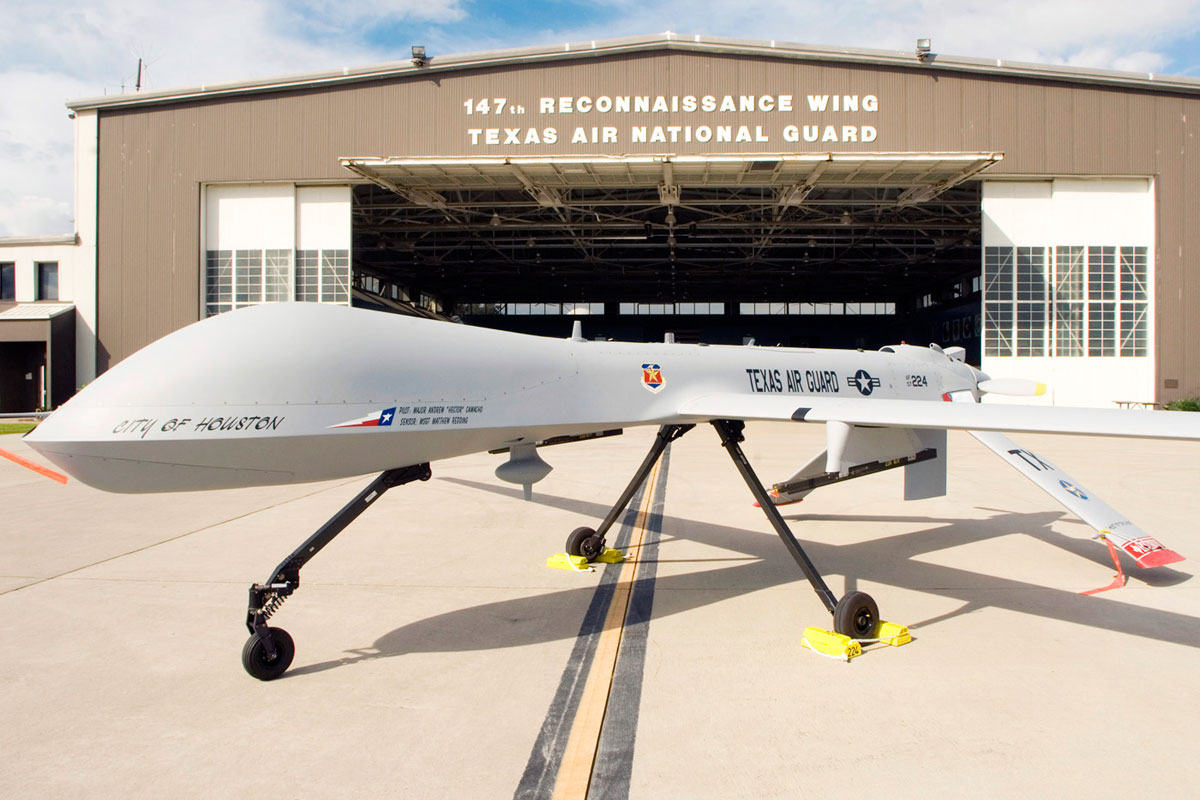
\includegraphics[width=1\linewidth]{predator.jpg}
		\caption{Внешний вид MQ-1 Predateor}
		\label{fig:predator1}
	\end{minipage}
	\begin{minipage}[h]{0.4\linewidth}
		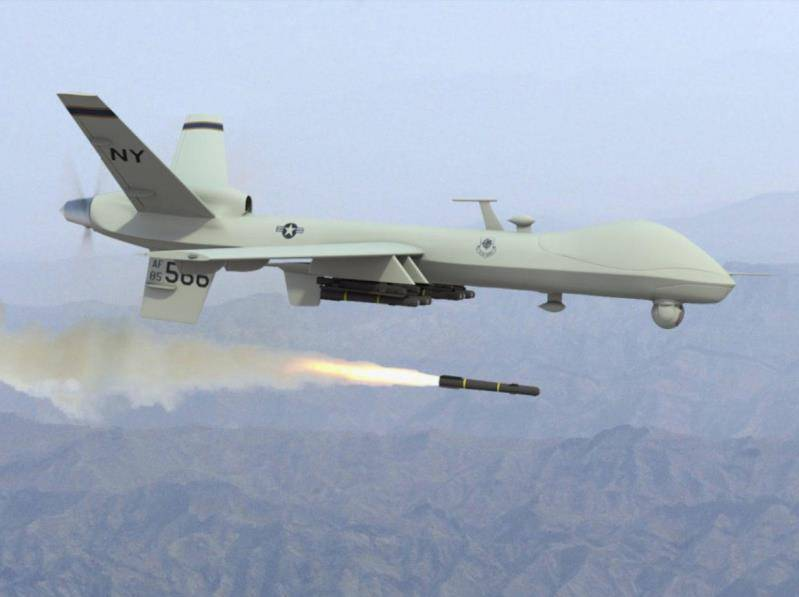
\includegraphics[width=1\linewidth]{reaper.jpg}
		\caption{Внешний вид MQ-9 Reaper}
		\label{fig:reaper1}
	\end{minipage}
\end{center}
\end{figure}

Остальные страны в той или иной степени повторяют опыт США – либо армии стран-партнеров напрямую закупают американские ударно-разведывательные беспилотные летательные аппараты, либо занимаются созданием близких по характеристикам БПЛА. К последним можно отнести китайский «Wing Loong» и российский «Дозор-600».

Особенностью вооружения данного класса БПЛА является то, что вооружение находится в основном на внешних подвесах, число которых сильно ограничено (у первых MQ-1 их было всего два – по штуке на крыло). Также важны весовые характеристики из-за ограниченной грузоподъемности БПЛА. Габаритами ПТУР определяется возможность закрепить на одном подвесе несколько ракет сразу.
\begin{figure}[h]
	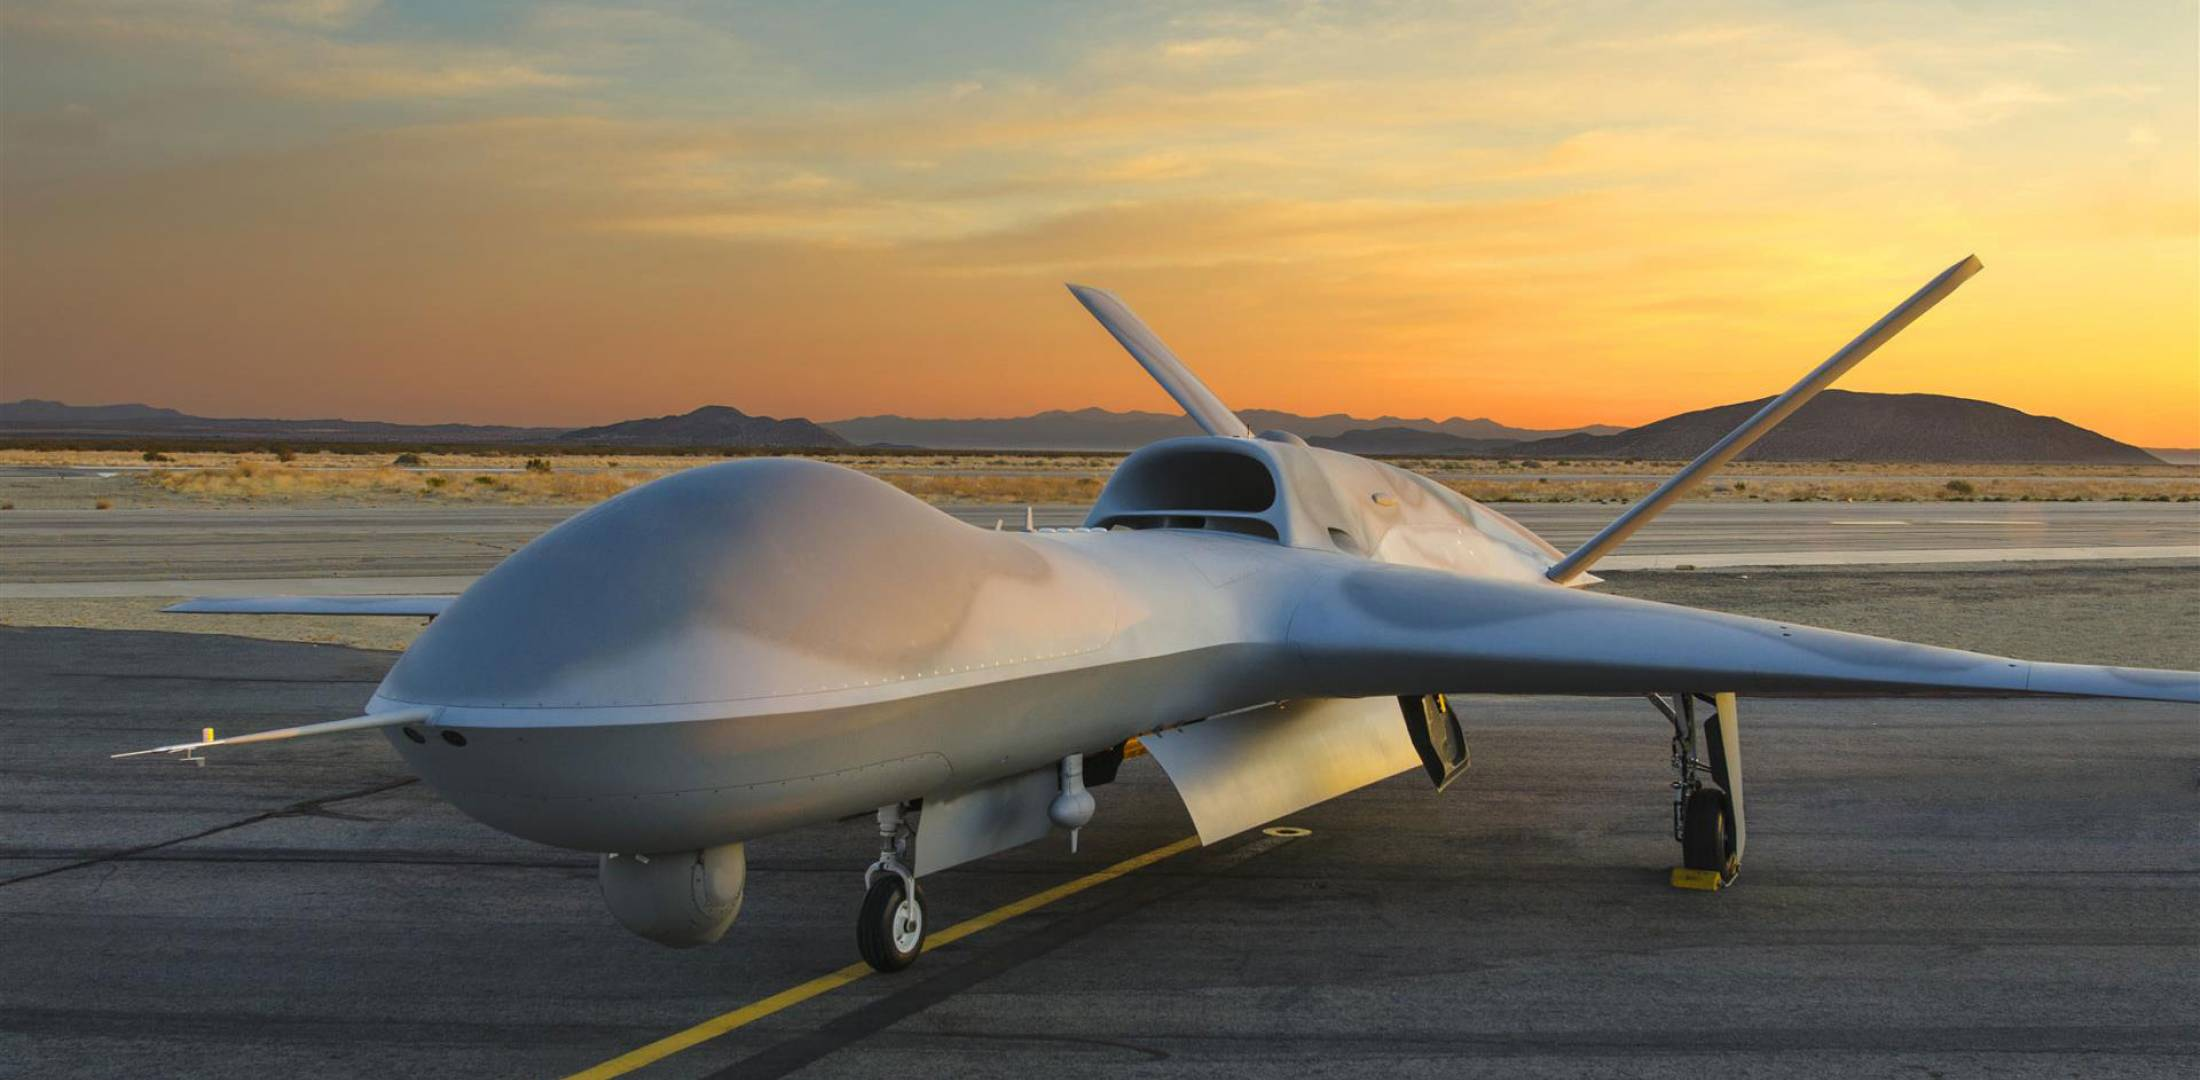
\includegraphics[width=\linewidth]{avenger.jpg}
	\caption{Внешний вид General Atomics Avenger}
	\label{fig:avenger1}
\end{figure}

Американский опыт демонстрирует следующее: сначала на MQ-1 устанавливали тяжелые и мощные ракеты AGM-114 Hellfire с лазерным наведением, однако военных не устроил малый боекомплект БПЛА и дороговизна каждой ракеты по сравнению с их типичными целями, а также количество сопутствующего ущерба, производимого каждым пуском мощного ПТУР (разрушение дорог и построек). Поэтому в скором времени после начала боевого применения кампания Raytheon разработала ПТУР AGM-176 Griffin меньшего калибра и массы. Теперь вместо двух ПТУР Hellfire БПЛА MQ-1 мог взять с собой шесть ПТУР Griffin, а ущерб от одного пуска не был столь разрушительным. Также AGM-176 имеет возможность наведения на цель по GPS и ИНС, что позволяет точно поражать неподвижные объекты без необходимости подсветки цели БПЛА.

\clearpage
\subsubsection{Влияние облика БПЛА \\на ТТХ используемых ПТУР}
Описанные выше особенности носителей ПТУР приводят к следующим требованиям:
\begin{enumerate}[1.]
	\item Необходимость наведения на цель, в том числе подвижную, по отраженному лазерному лучу;
	\item Максимальная дальность полета более 5 км при пуске с минимальной высоты;
	\item Возможность применения в тёмное время суток;
	\item Низкая заметность ПТУР во всех диапазонах для обеспечения как можно большей защищенности БПЛА от ПВО;
	\item Возможность наведения на цель при помощи GPS и/или ИНС;
	\item Малая масса и габариты, позволяющие БПЛА перевозить более 1 ПТУР на одном подвесе.
\end{enumerate}

\clearpage
\subsection{Облик современных танков}
Танки – самые защищенные из бронированных целей ракет БПЛА, поэтому тактико-технические характеристики этих ПТУР определяются, в основном, защищенностью современных и перспективных основных боевых танков.
Средства защиты танков сегодня можно разделить на 4 категории:
\begin{enumerate}[1.]
	\item Бронирование танка;
	\item Динамическая защита;
	\item Комплексы активной защиты (КАЗ):
	\begin{enumerate} [3.1.]
		\item Комплексы оптико-электронного противодействия (КОЭП);
		\item Системы с отстреливаемыми защитными зарядами.
	\end{enumerate}
\end{enumerate}

\subsubsection{Бронирование танка}
Броня – самый старый и естественный способ защиты экипажа и узлов боевой машины от поражения противником. В настоящее время стандартом танковой брони является комбинированная многослойная броня, состоящая из двух или более слоев металлических и неметаллических материалов. Такая броня разработана для защиты от кумулятивных боеприпасов и бронебойных оперенных противотанковых снарядов (БОПС).

Вне зависимости от действительного материала брони, показателем защищенности танка является так называемая эквивалентная толщина брони. Эквивалентная толщина – толщина листа гомогенной стали в миллиметрах, обеспечивающего такую же защищенность танка. Эту величину удобно использовать в расчетах эффективности различного вооружения против танка, а также при формировании ТТЗ на новые образцы вооружения.

На рисунке \ref{fig:leo2_armor} представлено бронирование современного танка ФРГ Леопард-2 в модификациях A0-A4. Данные модификации от последующих (в настоящий момент последней является A7V2) отличает полное отсутствие динамической защиты танка.

\begin{figure}[h]
	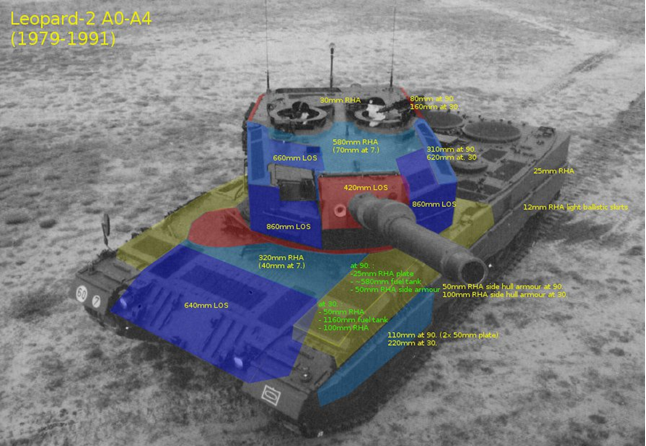
\includegraphics[width=\linewidth]{leo2_armor}
	\caption{Бронирование ОБТ Leopard-2 A0-A4}
	\label{fig:leo2_armor}
\end{figure}

Можно отметить крайне серьезное бронирование передней части крыши башни, однако задняя её часть бронирована слабее из-за наличия на ней приборов танка и люков экипажа.

Тенденция максимального бронирования передней части башни и корпуса и более слабого бронирования верхней проекции танка имела место всю историю танкостроения, и имеет место сейчас.

\subsubsection{Динамическая защита}
Динамическая защита (ДЗ)– более современный способ повышения защищенности танка. Суть ДЗ заключается в размещении поверх основной брони металлических контейнеров, содержащих элементы динамической защиты. Сегодня существует несколько разновидностей динамической защиты, большую их объединяет наличие в элементах ДЗ взрывчатого вещества, которое подрывается при разрушении контейнера и препятствует поражению носителя, снижая кинетическую энергию поражающего боеприпаса или разрушая кумулятивную струю. Такие системы, в основном, применяются на постсоветских танках.

Также существуют системы ДЗ, не содержащие в себе взрывчатого вещества. В этом случае снижение энергии поражающего боеприпаса достигается за счет механической энергии деформированных металлических пластин, содержащихся в ЭДЗ. Таким образом, достигается такой же эффект, как и в случае использования ДЗ со взрывчатым веществом.

На рисунках представлено размещение различных ЭДЗ на современных основных боевых танках.
Как можно заметить, в классических ОБТ с помощью динамической защиты так или иначе повышают защищенность бортов и лобовой части корпуса и башни. Отсутствие ДЗ, к примеру, на корме танка M1A2 Abrams (рисунок \ref{fig:abrams_armor}) с комплектом TUSK объясняется возможными негативными последствиями, которые оказывает срабатывание ДЗ на двигательную установку танка.
\begin{figure}[h]
	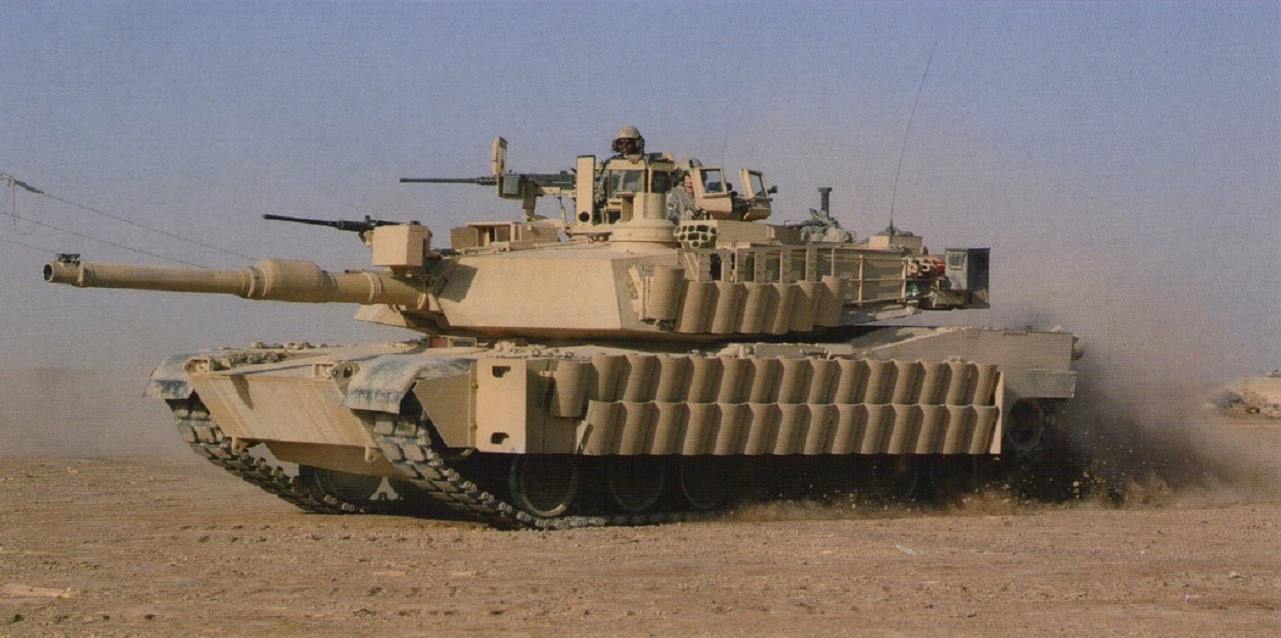
\includegraphics[width=\linewidth]{abrams_armor}
	\caption{Размещение элементов ДЗ на M1A2 Abrams\\с комплектом TUSK (США)}
	\label{fig:abrams_armor}
\end{figure}

По этим же причинам ограничено использование ДЗ на крыше танка, так как бронирование там слабее, чем на корпусе. Также на крыше располагается вспомогательное вооружение танка (зенитные пулеметы) и различные электронные средства, а также люки экипажа. Эту тенденцию можно наблюдать на классических танках Т-72 и Т-84У, схемы размещения элементов ДЗ на которых представлены на рисунках \ref{fig:t72_armor} и \ref{fig:oplot_armor} соответственно.

Таким образом, большинство современных ОБТ имеет слабость в защищенности верхней проекции как собственно броней, так и средствами динамической защиты.

Исключением из этого ряда является перспективный российский танк Т-14 «Армата»: так как башня у него необитаемая, вся её верхняя поверхность покрыта блоками ДЗ, которые можно увидеть на рисунке \ref{fig:armata_armor}.

\begin{figure}[h]
\begin{center}
	\begin{minipage}[h]{0.4\linewidth}
		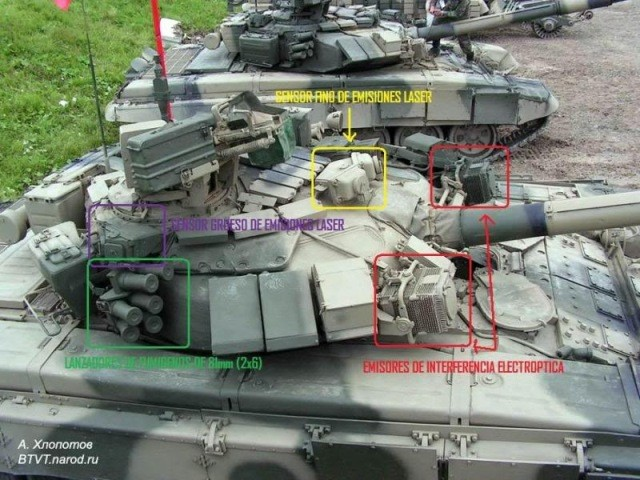
\includegraphics[width=1\linewidth]{t72_armor}
		\caption{Размещение элементов ДЗ на Т-72}
		\label{fig:t72_armor}
	\end{minipage}
	\begin{minipage}[h]{0.4\linewidth}
		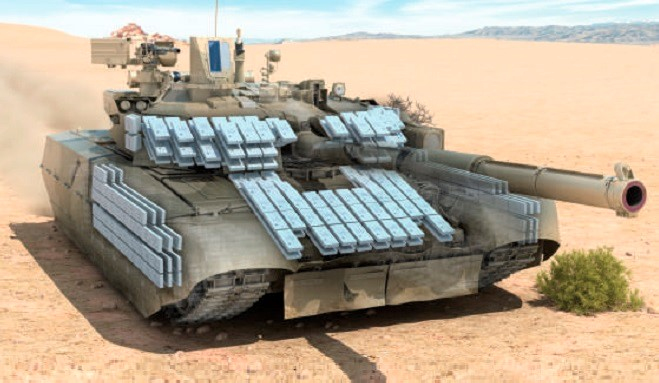
\includegraphics[width=1\linewidth]{oplot_armor}
		\caption{Размещение элементов ДЗ на Т-84У "Оплот" (Украина)}
		\label{fig:oplot_armor}
	\end{minipage}
\end{center}
\end{figure}

\begin{figure}[h]
\begin{center}
	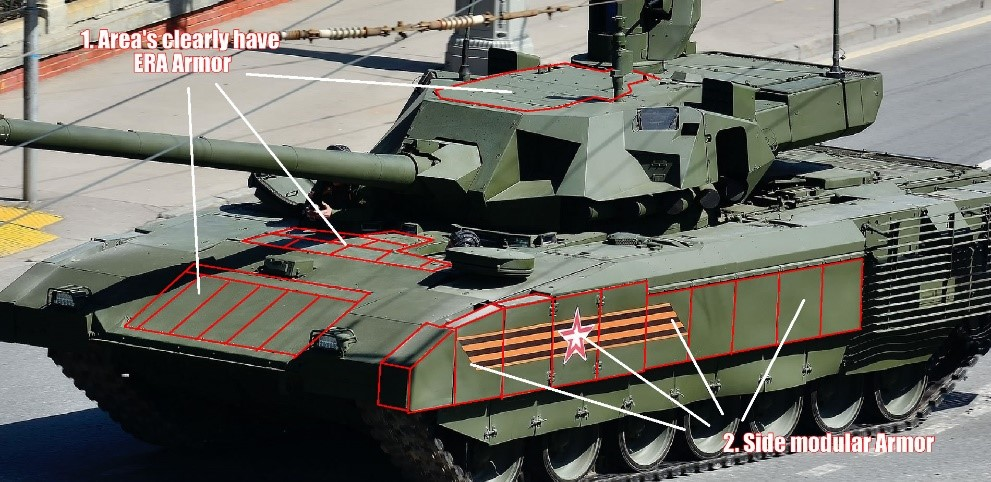
\includegraphics[width=\linewidth]{armata_armor}
	\caption{Размещение элементов ДЗ на Т-14 "Армата"}
	\label{fig:armata_armor}
\end{center}
\end{figure}
\subsubsection{Комплексы активной защиты}
Комплексы активной защиты (КАЗ) – системы, позволяющие обнаружить приближающийся противотанковый боеприпас и поставить помехи, уничтожающие цель или, по меньшей мере, сильно ослабить действие атакующего боеприпаса.

Как разновидность КАЗ, существуют системы оптико-электронного подавления, к ним относится российская «Штора-1». Данные системы позволяют подавлять координаторы наведения устаревших ПТУР – координаторы получают ложные сигналы от комплекса, и ракета врезается в землю или пролетает мимо. Такие системы эффективно работают против устаревших комплексов (Milan, HOT, «Малютка», «Конкурс» и т.д.), однако против новых систем они неэффективны. Поэтому на перспективные российские танки (Т-90СМ) данные системы уже не устанавливаются

Наибольшую опасность для противотанковых снарядов составляют КАЗ с отстреливаемыми элементами, к ним относятся комплексы «Дрозд», «Арена», Quick Kill, Trophy и т.д.
Большинство комплексов активной защиты защищает танк по кругу или части круга, оставляя для противотанковых боеприпасов возможность поразить танк сверху. Исключением из КАЗ, по некоторым данным, является израильский Trophy, создающий сплошную сферу вокруг танка, в которой подлетающие боеприпасы могут быть обнаружены и уничтожены. Однако вызывает вопросы низкий радиус действия Trophy – отстреливаемые элементы отстреливаются при подлете боеприпаса на расстояние порядка 2 м от танка, что, в случае использования, например, AGM-114 Hellfire с осколочно-фугасной БЧ, может означать повреждение внешних систем танка, включая сам комплекс Trophy.

\clearpage
\subsubsection{Влияние облика современных танков\\на ТТХ ПТУР}
Оптимальным способом поражения современных основных боевых танков является поражение их в верхнюю проекцию, так как
\begin{enumerate}[1.]
	\item Бронирование верхней проекции традиционно слабее лобового и бортового;
	\item Установка ДЗ на крышу затруднена и производится редко;
	\item Многие комплексы активной защиты не способны работать против боеприпасов, поражающих танк сверху.
\end{enumerate}

В случае использования в качестве носителя ПТУР ударно-разведывательного беспилотного летательного аппарата, задача поражения бронетехники сверху упрощается в связи с положением носителя при стрельбе.
Таким образом, особенности целей ПТУР приводят к следующим требованиям:
\begin{enumerate}[1.]
	\item Необходимость реализации манёвра для поражения целей в верхнюю проекцию;
	\item Бронепробитие на уровне 800 мм по нормали.
\end{enumerate}

\clearpage
\subsection{Обзор существующих образцов ПТУР,\\применяемых на БПЛА}
Так как основным разведывательно-ударным БПЛА, несущим на себе противотанковое вооружение, является Predator и его копии и модификации, основным противотанковым средством таких БПЛА является классический ПТУР AGM-114 Hellfire и более современный ПТУР AGM-176 Griffin.

Страны, напрямую не эксплуатирующие американские ударно-разведывательные БПЛА, вооружают свои образцы похожими по своим характеристикам противотанковыми управляемыми ракетами. В частности, Китайский ударно-разведывательный беспилотный летательный аппарат Wing Loong вооружен идентичным Hellfire по массе, калибру и системе наведения ПТУРом AFT10 (HJ-10), который ранее устанавливался на боевые вертолеты.
\subsubsection{AGM-114 Hellfire}
Данный образец выбран в качестве вооружения ударно-разведывательных беспилотных летательных аппаратов, так как им же вооружаются ударные вертолеты США.
ПТУР представлен в разрезе на рисунке \ref{fig:hellfire1}.
\begin{figure}[!h]
\begin{center}
	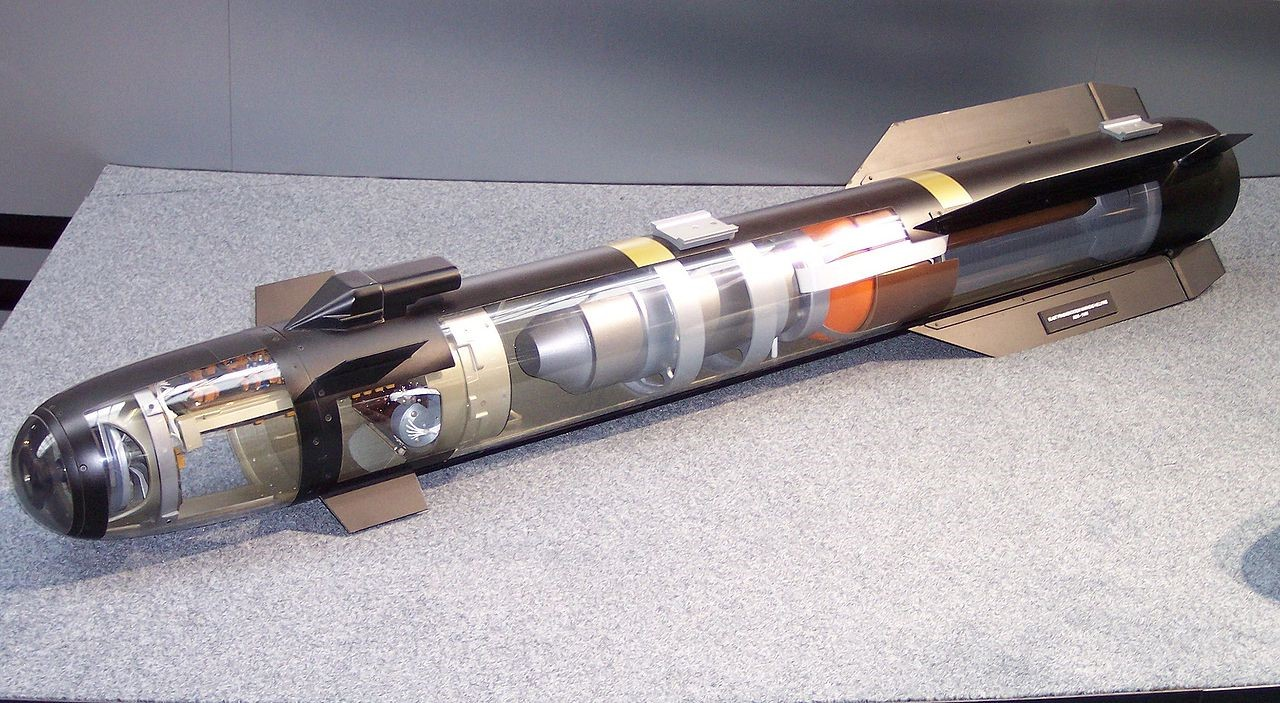
\includegraphics[height=7cm]{hellfire1}
	\caption{AGM-114 Hellfire}
	\label{fig:hellfire1}
\end{center}
\end{figure}
ТТХ образца представлены в таблице \ref{tab:hellfire_stats}
\begin{table}[!h]
	\begin{center}
		\caption{ТТХ ПТУР AGM-114 Hellfire}
		\begin{tabular}{|l|l|}
  		\hline
		Калибр, мм & 178 \\ \hline
		Стартовая масса, кг	& 50 \\ \hline
		Тип БЧ	& Кумулятивная \\ \hline
		Система наведения & Полуактивная лазерная ГСН \\ \hline
		Масса БЧ, кг & 9 \\ \hline
		Максимальная дальность, км & 20 \\ \hline
		Максимальная скорость, м/с & 440 \\ \hline
		Год принятия на вооружение & 1984 \\ \hline
		\end{tabular}
		\label{tab:hellfire_stats}
	\end{center}
\end{table}

\subsubsection{AGM-176 Griffin}
Данный образец изначально разрабатывался как недорогая система, использующая в себе наработки предыдущих образцов: FGM-148 Javelin и AIM-9X Sidewinder. За счет уменьшения калибра по сравнению с Hellfire, разработчики добились уменьшения сопутствующего ущерба при применении ПТУР, а также обеспечили возможность крепления трех ПТУР на одном внешнем подвесе MQ-1 Reaper.

Также данный ПТУР, в отличие от предшественника, можно наводить на неподвижные цели с помощью ИНС и GPS.

Внешний вид ПТУР представлен на рисунке \ref{fig:griffin1}
\begin{figure}[!h]
	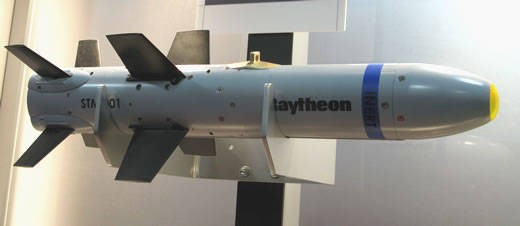
\includegraphics[width=\linewidth]{griffin}
	\caption{AGM-176 Griffin}
	\label{fig:griffin1}
\end{figure}

ТТХ образца представлены в таблице \ref{tab:griffin_stats}
\begin{table}[!h]
	\begin{center}
		\caption{ТТХ ПТУР AGM-176 Griffin}
		\begin{tabular}{|l|l|}
  		\hline
		Калибр, мм & 140 \\ \hline
		Стартовая масса, кг & 20 \\ \hline
		Тип БЧ & Кумулятивная \\ \hline
		Система наведения & Полуактивная лазерная ГСН, GPS, ИНС \\ \hline
		Масса БЧ, кг & 5.9 \\ \hline
		Максимальная дальность, км & 18 \\ \hline
		Максимальная скорость, м/с & дозвуковая \\ \hline
		Год принятия на вооружение & 2008 \\ \hline
		\end{tabular}
		\label{tab:griffin_stats}
	\end{center}
\end{table}
\subsection{Вывод}
В настоящее время разведывательно-ударные БПЛА являются серьезным средством борьбы с танками противника из-за своей относительной дешевизны и отсутствии риска для оператора. Современные ПТУР, которые устанавливаются на такие беспилотные летательные аппараты, могут иметь меньшую массу и габариты по сравнению с ПТРК, запускаемыми с поверхности земли из-за более слабой защищенности их целей в верхней проекции. Также уменьшение калибра позволяет снизить стоимость ракеты, увеличить объем вооружения БПЛА и снизить сопутствующий ущерб при применении комплекса в целом.

Выработанные требования к ТТХ проектируемого ПТУР:
\begin{enumerate}[1.]
	\item Реализация маневра для поражения целей в верхнюю проекцию
	\item Возможность наведения на цель, в том числе подвижную, с помощью полуактивной лазерной ГСН по отраженному лучу или активной ГСН
	\item Бронепробитие на уровне 800 мм по нормали
	\item Максимальная дальность полета более 4 км с минимальной высоты пуска
	\item Низкая заметность во всех диапазонах
	\item Возможность применения в темное время суток
\end{enumerate}

\clearpage
\section{Устройство комплекса}
В состав авиационного комплекса вооружения входят:
\begin{enumerate}[1.]
	\item БПЛА – носитель.
	\item Дозвуковая противотанковая управляемая ракета.
\end{enumerate}

Ракета состоит из трёх отсеков. Первый отсек – полуактивная лазерная головка самонаведения, закрытая прозрачным обтекателем. Во втором отсеке находится кумулятивная боевая часть, взрыватель, ботовая система управления и батареи питания. Четвертый отсек – твердотопливная двигательная установка.

Конструкция ракеты модульная, поэтому каждый отсек может быть заменен независимо от всего изделия. Отсеки друг с другом соединяются винтами.
\subsection{Устройство отсеков ПТУР}
\emph{Отсек 1. Инфракраснaя лазерная головка самонаведения.}

Головка самонаведения имеет обтекатель оживальной формы, прозрачный для ИК-лучей, и состоит из координатора и электронного блока. Головка самонаведения соединена с блоком управления проводами, уложенными в гаргрот.

\emph{Отсек 2. Боевая часть и система управления.}

Система управления и батарея созданы в виде одного блока и устанавливаются в отсек в первую очередь. Далее, после монтирования индукционных рулевых машинок и взрывателя, в ПТУР вкладывается кумулятивная боевая часть. После монтажа боевой части, к ПТУР прикручивается головка самонаведения, предварительно соединенная кабелями блоком управления. Также в блоке управления есть разъем для кабеля, по которому поступает сигнал от носителя.

\emph{Отсек 3. Двигательная установка.}

Двигатель – твердотопливный одноступенчатый. После отделения ракеты от носителя он обеспечивает её разгон до маршевой скорости. Далее ракета управляется с помощью аэродинамических рулей и поражает цель с выключенным двигателем.

\emph{Планер.}

Рули и крылья ПТУР расположены в одних плоскостях; по аэродинамической схеме «утка». Корпус ПТУР выполнен из лёгкого дюралевого сплава, способного выдержать нагрузки при полёте.

\subsection{Описание работы комплекса}
Пуск и управляемый полет ПТУР осуществляются следующим образом. После обнаружения системой поиска (дальность 10 км), находящейся на БПЛА, беспилотник направляется к цели для её поражения. У оператора комплекса есть достаточное время, зависящее от высоты, для принятия решения о пуске. Решение о пуске можно принять после сокращения расстояния между БПЛА и целью до максимальной дальности применения ПТУР. Также перед пуском оператору необходимо начать подсветку цели лазером, находящемся на борту БПЛА,

Далее ПТУР производится запуск ПТУР. ГСН ракеты после пуска должна захватить цель. Автопилот начинает работать уже на этом этапе, однако скорость не позволяет ракете маневрировать за счёт аэродинамических органов управления. РДТТ отрабатывает и разгоняет её до максимальной скорости (300-315 м/с). Во время работы двигателя поток, набегающий на ПТУР позволяет органам управления контролировать полёт и осуществлять управление ракетой. После отработки РДТТ (3.9 сек) ракета летит до цели с постоянной скоростью порядка 270 м/с. Постоянство скорости обеспечивается законом наведения. Детонация БЧ осуществляется при контакте с целью.

На рисунке \ref{fig:complex_work_scheme} наглядно представлена схема работы комплекса.
\clearpage
\begin{figure}[!h]
	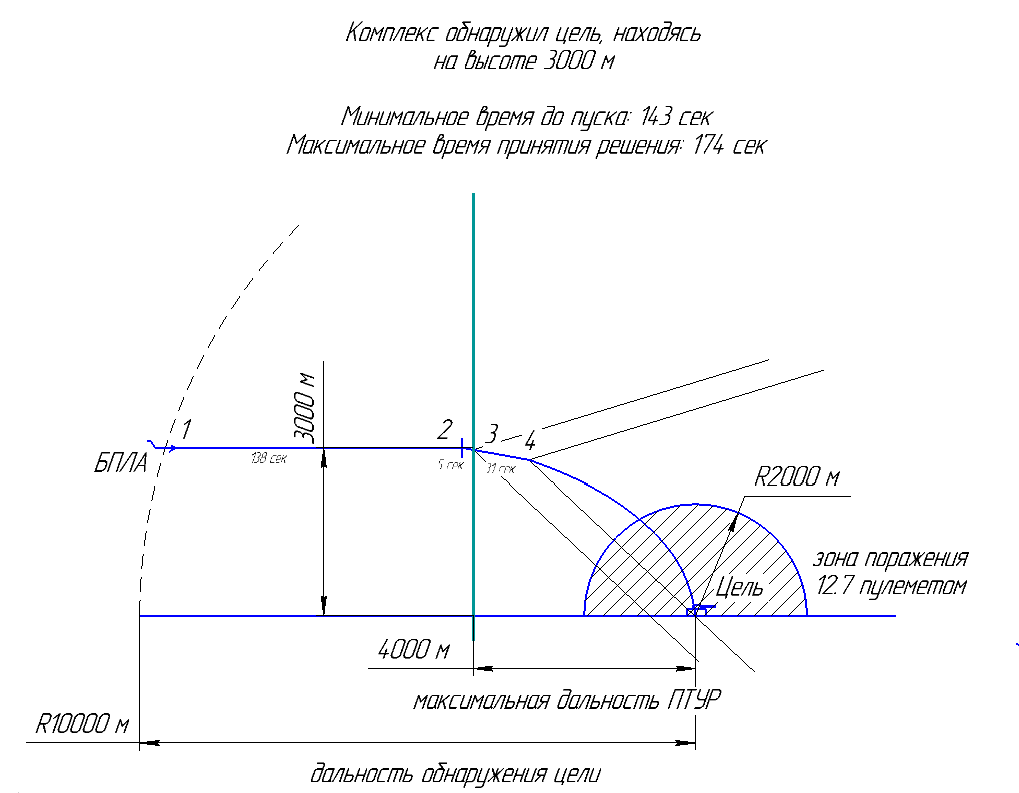
\includegraphics[width=\linewidth]{complex_works}
	\caption{Схема работы комплекса}
	\label{fig:complex_work_scheme}
\end{figure}


1 – цель попала в зону обнаружения БПЛА. Комплекс начинает движение в сторону цели;

2 – БПЛА выходит на пикирующий курс, позволяющий ПТУР быть направленной на цель после отделения;

3 – цель находится в зоне действия ПТУР, оператор БПЛА может принимать решение о запуске;

4 – цель находится в предельном положении, позволяющем ГСН ПТУР захватить цель после пуска. После выхода из этого положения пуск совершать не следует.

\clearpage
\subsection{Описание метода наведения ПТУР}
Для поражения цели сверху нужно применять особый метод наведения, так как «обычные» методы, например метод чистой погони, не позволят получить траекторию нужной формы.

В данном комплексе применяется метод погони с упреждением. Головка самонаведения обеспечивает угол обзора в 60 градусов. При отделении угол пеленга, обозначаемый $\alpha$, устанавливается максимальным значением вне зависимости от дальности. В зависимости от расстояния от точки пуска до цели, системой управления БПЛА просчитывается $t_{\text{нач}}$ и $t_{\text{кон}}$, которыми задается длительность манёвра и время его начала.
\begin{figure}[!h]
	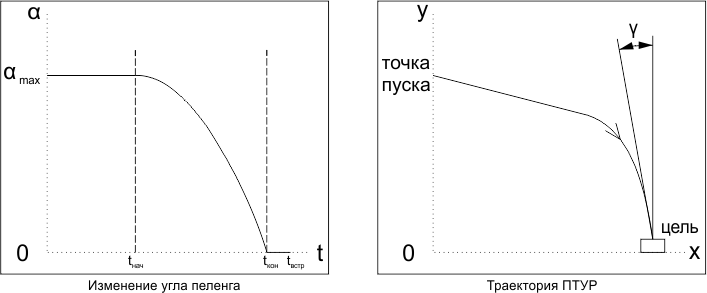
\includegraphics[width=\linewidth]{pre_hit_target}
	\caption{Изменение угла пеленга и траектория ПТУР}
	\label{fig:pre_hit_target}
\end{figure}

За счёт этого удается получить достаточно крутую траекторию и поразить цель в верхнюю проекцию. Важным критерием успешного поражения в данном случае является угол встречи с целью к вертикали, обозначаемый $\gamma$. Вид закона изменения угла пеленга и траектории представлен на рисунке \ref{fig:pre_hit_target}.

Определение оптимальных с точки зрения перегрузок, действующих на ПТУР, момента начала уменьшения угла пеленга уменьшения и скорости уменьшения – задача оптимизации, так как при слишком резком уменьшении пеленга ракета будет испытывать большие поперечные перегрузки, а при слишком слабом траектория будет слишком пологой и угол $\gamma$ может помешать её поражению. Решение этой задачи подробно описано в пункте \ref{chapter:traectory_optimization}.

В случае движения цели, целесообразно производить наведение в упрежденную точку, а в конце манёвра переводить наводить лазер на цель.
Наличие ГСН позволяет бороться с влиянием на поражение цели случайных возмущений, например ветра.

\clearpage
\section{Баллистическое проектирование ПТУР}
При решении задачи внешней баллистики определяются основные характеристики образца, которые должны соответствовать требованиям технического задания. В качестве основного критерия принимается минимум стартовой массы, при которой образец реализует доставку полезной нагрузки на необходимую дальность. При уменьшении веса ПТУР уменьшаются и ее габариты, что позволяет уменьшить расход материалов и затраты на изготовление конструкции образца.
\subsection{Исходные данные}
Исходные данные назначены в соответствии с классом разрабатываемого образца – ПТУР «воздух - поверхность» с силовой установкой РДТТ. Данные приведены в таблице \ref{tab:bal_proekt_nu}.

\begin{table}[!h]
	\begin{center}
		\caption{Исходные данные для баллистического проектирования}
		\begin{tabular}{|l|l|}
  		\hline
Дальность полета, км & 4000 \\ \hline
Высота пуска, км & 500 .. 4000 \\ \hline
Скорость пуска, км/ч & 150 км/ч \\ \hline
Число Маха на маршевом участке, M & 0,88 \\ \hline
		\end{tabular}
		\label{tab:bal_proekt_nu}
	\end{center}
\end{table}

В ходе баллистического проектирования ставится задача выбора оптимальной траектории ПТУР для полета на максимальную дальность. Для этого проварьируем высоты маршевого участка от 500 до 4000 м с шагом в 500 м. Лучший вариант будем определять по значению массы АУР, полученной при баллистическом проектировании.

Для образца на этапе баллистического проектирования совместно с решением задачи внешней баллистики проводится расчет параметров РДТТ, для чего необходимо располагать всей информацией о нем.

\subsection{Назначение параметров}
Калибр ПТУР назначаем из соотношения бронепробития и калибра, характерного для современных ПТУР:
\[ B = 6..8 \cdot d \]

Таким образом, $d = 800/6.8 = 117,7 \text{ мм}$. Принимаем диаметр кумулятивной воронки $d = 120 \text{ мм}$. Зная калибр ПТУР,
\begin{itemize}
	\item масса боевой части $m_{\text{бч}} = 2,2 \text{ кг}$;
	\item масса системы управления $m_{\text{су}} = 4,5 \text{ кг}$;
	\item масса полезной нагрузки $m_{\text{пн}} = m_{\text{бч}} + m_{\text{су}} = 6,7 \text{ кг}$;
	\item конструктивно-весовая характеристика $\beta = 1,4$;
	\item средняя скорость полета $V_{\text{ср}} = 290 \text{ м/с}$;
	\item тяговооруженность на стартовом участке $\eta_0 = 6$;
	\item удельный импульс топлива:    $I_{10} = 2400 \text{ (Н*с)/кг}$.
\end{itemize}
Параметры атмосферы принимаем принять постоянными невозможно, так как широк диапазон применения ПТУР по высоте. Давление, плотность и скорость звука в зависимости от высоты принимаем по ГОСТ 4401-81 (стандартная атмосфера).

\subsection{Система уравнений для решения\\задачи внешней баллистики}
Описание используемой системы уравнений подробно дано в пункте 7.4.1.

Системы уравнений записаны с учетом следующих допущений:
\begin{enumerate}[1.]
	\item Движение образца происходит в одной плоскости (вертикальной).
	\item Работа органов управления считается идеальной.
	\item Кривизна Земли и переменность ускорения свободного падения не учитываются.
	\item Движение образца описывается движением его центром масс (образец рассматривается как тяжелая материальная точка).
\end{enumerate}
\clearpage
Начальные условия для интегрирования на первом участке траектории:
\begin{itemize}
	\item t = 0 сек; V = 150 м/с (скорость носителя);
	\item х = 0 м; y = 3000 м (высота пуска);
	\item $\mu$ = 0.
\end{itemize}
Начальные условия для остальных участков определяются в результате расчетов на предыдущих участках.

Для решения задачи на активном участке траектории используется система уравнений (\ref{system:active}).

\begin{equation}
	\label{system:active}
	\left\{
			\begin{aligned}
			\frac{dV}{dt} & = \frac{g \cdot \eta}{1 - \mu} - i \cdot C_{43} \left( \frac{V}{\alpha(Y)} \right) \cdot \frac{\rho(Y)V^2g}{2q_{m0}(1-\frac{g*\eta}{J_{10}})} - g\sin \left[ \arctg \left( \frac{Y-Y_{\text{ц}}}{X-X_\text{ц}} \right) \right] ; \\
			\frac{dX}{dt} & = V \cdot \cos x  \left[ \arctg \left( \frac{Y-Y_{\text{ц}}}{X-X_\text{ц}} \right) \right] ; \\
			\frac{dY}{dt} & = V \cdot \sin x  \left[ \arctg \left( \frac{Y-Y_{\text{ц}}}{X-X_\text{ц}} \right) \right] .\\
			\frac{dm}{dt} & = \frac{g \cdot \eta}{J_{10}}
			\end{aligned}
	\right.
\end{equation}
Здесь $\alpha(t)$ - закон изменения угла пеленга; X, Y - текущие координаты ПТУР; $X_\text{ц}$, $Y_\text{ц}$ - координаты цели; $V$ - скорость ПТУР; $\eta$ - тяговооруженность; $\mu = \frac{dm}{dt}$ - расход топлива; $J_{10}$ - единичный импульс топлива; $a(Y)$ - скорость звука в зависимости от высоты полета; $C_{43}$ - функция 1943 года для определения лобового сопротивления ЛА.


Для решения задачи на пассивном участке траектории используется система уравнений (\ref{system:passive}).
\begin{equation}
	\label{system:passive}
	\left\{
			\begin{aligned}
			\frac{dV}{dt} & =  - i \cdot C_{43} \left( \frac{V}{\alpha(Y)} \right) \cdot \frac{\rho(Y)V^2g}{2q_{m0}} - g\sin \left[ \arctg \left( \frac{Y-Y_{\text{ц}}}{X-X_\text{ц}} \right) \right] ; \\
			\frac{dX}{dt} & = V \cdot \cos x  \left[ \arctg \left( \frac{Y-Y_{\text{ц}}}{X-X_\text{ц}} \right) \right] ; \\
			\frac{dY}{dt} & = V \cdot \sin x  \left[ \arctg \left( \frac{Y-Y_{\text{ц}}}{X-X_\text{ц}} \right) \right] .\\
			\frac{dm}{dt} & = 0
			\end{aligned}
	\right.
\end{equation}

На этапе баллистического проектирования величина $\alpha(t)$ (закон изменения угла пеленга) изменяется по закону, описанному в уравнении (\ref{system:rough_alpha}). На этапе баллистического проектирования проверяется соответствие диаграммы скорости требуемой форме и способность ПТУР поразить цель на максимальной дальности, поэтому закон $\alpha(t)$ выражен в виде кусочной линейной функции с произвольными участками.
\begin{equation}
	\label{system:rough_alpha}
	\alpha(t) = \begin{cases}
		25 & \text{, если t < 15} \\
		25 \cdot \dfrac{21 - t }{21-15} &  \text{, если } 15 \le t < 21 \\
		0 &  \text{, если t } \ge 21\\
	\end{cases}
\end{equation}

Изучение влияния $\alpha(t)$ на форму траектории и эффективность пражения цели более подробно описано в разделе \ref{chapter:traectory_optimization} на странице \pageref{chapter:traectory_optimization}.

\subsection{Результаты баллистического проектирования}
Результаты проектирования:
\begin{itemize}
	\item Стартовая масса ракеты:     m = 9,8 кг;
	\item Относительный запас топлива:    $\mu_0$ = 0,25;
	\item Запас топлива:       $\omega_0$ = 1,3 кг;
	\item Продолжительность стартового участка:  $t_0$ = 4.5 c;
	\item Секундный расход топлива:    $G_0$ = 0,31 кг;
	\item Средняя скорость полета:     $V_{\text{ср}}$ = 280,2 м/с;
	\item Начальная скорость:      $V_0$ = 42,0 м/с;
	\item Среднее время полета:     $t_\text{к}$ = 17,3 с;
	\item Потребная тяга:      $P_0$ = 680 Н;
	\item Полный импульс:      $I_P$ = 3300 Н $\cdot$ с.
\end{itemize}

Для старта с высоты 3100 м и расстояния до цели 4000 м приведена траектория полета движения (рисунок \ref{fig:sample_traectory}), a также графики изменения скорости ПТУР (рисунок \ref{fig:sample_speed}) и изменения угла пеленга (рисунок \ref{fig:sample_peleng}).
\clearpage

\begin{figure}[!h]
\begin{center}
	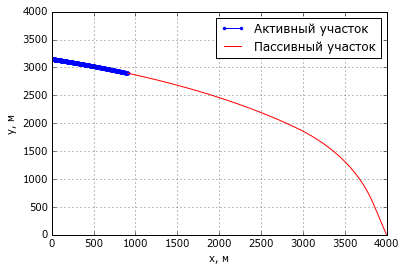
\includegraphics[height=8cm]{sample_traectory}
	\caption{Одна из возможных траекторий движения ПТУР}
	\label{fig:sample_traectory}
\end{center}
\end{figure}

\begin{figure}[h]
\begin{center}

	\begin{minipage}[h]{0.47\linewidth}
		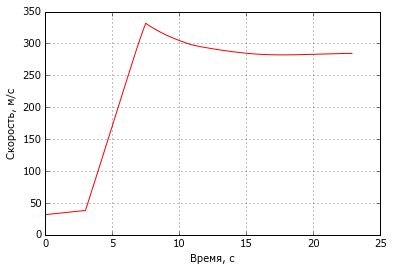
\includegraphics[width=1\linewidth]{sample_speed}
		\caption{Один из возможных графиков $V(t)$}
		\label{fig:sample_speed}
	\end{minipage}
	\hfill
	\begin{minipage}[h]{0.47\linewidth}
		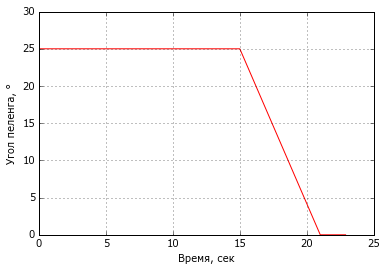
\includegraphics[width=1\linewidth]{sample_peleng}
		\caption{Принятая зависимость $\alpha(t)$}
		\label{fig:sample_peleng}
	\end{minipage}
\end{center}
\end{figure}

Графики отражают соответствие баллистического проектирования исходной задаче баллистического проектирования.

\clearpage
\section{Проектирование РДТТ}
На данном этапе проектирования ставится задача выбора конструктивных параметров двигательной установки стартовой ступени. В качестве топлива было выбрано нитраминное смесевое ТРТ (состав №13). Корпус ДУ выполнен из материала СП-33.

\subsection{Исходные данные}
Исходные данные основаны на результатах баллистического проектирования. В результате, были назначены следующие исходные данные:
\begin{itemize}
	\item Наружный диаметр корпуса ДУ:				$D_\text{н}$ = 125 мм;
	\item Полный импульс тяги стартового двигателя: $I_\text{п}$ = 3300 Н $\cdot$ c;
	\item Время работы двигателя:					$t_0$ = 4,5 с;
	\item Масса топлива двигателя:					$\omega_0$ = 1,3 кг;
\end{itemize}

\emph{Характеристики топлива (нитраминное смесевое ТРТ):}

\begin{itemize}
	\item Массовые доли и плотности компонентов топлива:
	\begin{enumerate}[1.]
		\item НТРВ:  		$g_1$ = 0,12; 		$\delta_1$ = 920  $\text{кг/м}^3$;
		\item ПХА:			$g_2$ = 0,62;		$\delta_2$ = 1950 $\text{кг/м}^3$;
		\item НМХ:			$g_3$ = 0,08;		$\delta_3$ = 1900 $\text{кг/м}^3$;
		\item Al:			$g_4$ = 0,18;		$\delta_4$ = 2700 $\text{кг/м}^3$;
	\end{enumerate}
	\item Плотность топлива:			$\delta=1/\sum_{i=1}^n \frac{g_i}{\delta_i} $=1794.8  $\text{кг/м}^3$;
	\item Тепловой эффект реакции:				Q = 5831,1 кДж/кг;
	\item Единичный импульс топлива:				$J_{40/1}$ = 2605,74 м/с;
	\item Температура продуктов сгорания:			$T_0$ = 3448,9 К;
	\item Показатель адиабаты:					k = 1,1821;
	\item Газовая постоянная газовой фазы:			$R_\text{г}$ = 428,77 Дж/кг $\cdot$ К;
	\item Массовая доля к-фазы в продуктах сгорания:	Z = 0,31947;
	\item Газовая постоянная смеси:		$R = R_\text{г}\cdot(1−Z)$ = 291,791 Дж/кг $\cdot$ К;
	\item Закон скорости горения:	$\xi=Z/(1-Z)=0,469$;
	\item Скорость горения при $p_{ref}$ = 5МПа:	$	u_{ref}$=6.0  мм/с;
	\item Показатель в степени закона горения:		$\nu$=0.25;
	\item Единичная скорость горения: $u_1=u_{ref} / p_{ref}^\nu$ = 4.012  мм/с;
	\item Термохимическая константа:				$D_t$=0.0025  1/($\textdegree$C);
\end{itemize}

\emph{Характеристики материала корпуса ДУ (СП-33):}

\begin{itemize}
	\item Плотность материала					$\rho_\text{м}=7830  \text{кг/м}^3$ ;
	\item Временное сопротивление				$\sigma_\text{вр}=1650$ МПа ;
	\item Условный предел текучести			$\sigma_{0,2}=1350$ МПа ;
	\item Минимальная технологическая толщина стенки	$\delta_{min}$=1,5 мм;
\end{itemize}


\emph{Характеристики ТЗП:}

\begin{itemize}
	\item Плотность $\rho_\text{u}=1500  \text{кг/м}^3$ ;
	\item Толщина $\delta_u$=2,5 мм;
\end{itemize}

Расчет параметров ДУ приведен в Приложении Б (страница \ref{chapter:appendix2}).

При выборе наилучшего варианта ДУ в качестве основного критерия использовалась общая масса ДУ. В процессе сужения области поиска наилучшего решения во внимание принимались значения удельного импульса $I_{\text{уд}}$ и массы твердого топлива

\subsection{Результаты проектирования РДТТ}
Ниже представлены параметры выбранного варианта ДУ:
\begin{itemize}
	\item Давление в камере сгорания:				p = 7,6 МПа;
	\item Масса твердого топлива:					$\omega$ = 1.36 кг; 
	\item Удельный импульс:						$I_{10}$ = 2482 м/с; 
	\item Диаметр критического сечения сопла:			$d_{\text{кр}}$ = 10  мм; 
	\item Диаметр выходного сечения сопла:				$d_{\text{вых}}$ = 84 мм;
	\item Масса конструкции ДУ:					$m_{\text{кду}}$ = 2,5 кг; 
	\item К-т конструктивно-весового совершенства ДУ:		$\alpha$ = 0,289; 
	\item Толщина стенки корпуса ДУ:					$\delta$ = 1,5 мм; 
	\item Толщина слоя ТЗП:						$\delta u$ = 2,5 мм; 
	\item Минимальная толщина горящего свода заряда:		$e_1$ = 23 мм;
	\item К-т заполнения поперечного сечения заряда:		$\epsilon$ = 0,77.
\end{itemize}


\clearpage
\section{Аэродинамическое проектирование}
\subsection{Выбор аэродинамической схемы}
Основа выбора – анализ существующих схем: нормальной, утки, бесхвостки и поворотного крыла.

Для планеров, которым необходимо маневрировать на низких высотах рациональна компоновка в схеме «утка», в связи с тем, что данная схема обеспечивает лучшую манёвренность и управляемость.

\subsection{Центровочный расчет}
Центровкой называется процесс размещения грузов по корпусу изделия. При этом определяются центр тяжести, разбежка центра тяжести и моменты инерции изделия. В результате расчетов двигательной установки и предварительного проектирования образца была получена длина корпуса ракеты, равная L = 940 мм.

В таблице \ref{tab:center} приведены массы, длины и координаты центров тяжести отсеков ракеты. Координаты центра тяжести отсчитываются от носка корпуса. Также в таблице приведены весовые характеристики топлив каждой из двигательных установок.

\begin{table}[!h]
	\begin{center}
		\caption{Расрпеделение массы ПТУР по отсекам}
		\begin{tabular}{|l|p{25mm}|p{3cm}|p{35mm}|p{35mm}|}
  		\hline
№ &	Название отсека	& Масса отсека, m, кг & Длина отсека, l, мм & Центр тяжести отсека, X, мм \\ \hline
1 &	ГСН	& 0,8	& 172	& 130 \\ \hline
2 &	БЧ	& 3,1	& 205	& 305 \\ \hline
3 &	СУ и РМ	& 2,9	& 216 &	505 \\ \hline
4 &	РДТТ	& 2,5	& 288 &	690 \\  \hline
5 &	Сопловой блок	& 0,7	& 110 & 	820 \\ \hline
6 &	Топливо РДТТ	& 1,4 &	110	& 379 \\ \hline
		\end{tabular}
		\label{tab:center}
	\end{center}
\end{table}

\clearpage
\emph{Результаты центровочного расчета:}
\begin{itemize}
	\item Стартовая масса образца:					$m_0$ = 9,8 кг;
	\item Масса ракеты в конце активного участка:	$m_1$ = 8,4 кг;
	\item Центр тяжести ракеты на старте:			$X_{\text{цт полн}}$ = 488 мм;
	\item Центр тяжести «пустой» ракеты:			$X_{\text{цт пуст}}$ = 432 мм;
	\item Разбежка центра тяжести:					$\Delta X_\text{цт}$ = 57 мм;
	\item Относительная разбежка центра тяжести (\%):	$\Delta X_\text{цт}$ = 6,33\%;
	\item Момент инерции планера на старте:			$J_\text{z полн}$ = 931 Н$\cdot \text{м}^2$;
	\item Момент инерции «пустого» планера:			$J_\text{z пуст}$ = 604 Н$\cdot \text{м}^2$.
\end{itemize}

\subsection{Выбор геометрии планера}
В результате проектирования были получены следующие геометрические параметры планера:
\begin{itemize}
	\item Длина фюзеляжа:						$l_\text{ф} $ = 940 мм;
	\item Диаметр фюзеляжа:						d = 125 мм;
	\item Площадь миделева сечения:				$S_\text{м} $ = 0,012 м2;
	\item Длина головной части корпуса:			$l_\text{гч} $ = 172 мм;
	\item Длина кормовой части корпуса:			$l_\text{кч} $ = 768 мм;
	\item Удлинение фюзеляжа:					$\lambda_\text{ф} $ = 7,2;
	\item Удлинение головной части фюзеляжа:	$\lambda_\text{гч} $ = 1,37;
	\item Удлинение кормовой части фюзеляжа:	$\lambda_\text{кч} $ = 5,86;
	\item Сужение кормовой части фюзеляжа:		h = 0.
\end{itemize}

Определим площадь крыла исходя из величины потребной перегрузки и максимального угла атаки. Предельная перегрузка необходимая для маневра горка у подобного класса ракет обычно не превышает значения 6g. Поэтому примем:
\begin{itemize}
	\item Потребная перегрузка:					            $h_\text{потр}$ = 6;
	\item Максимальный угол атаки ЛА:			                $\alpha = 6\textdegree$;
	\item Средняя скорость полета:				            $V_\text{ср}$ = 280 м/с;
	\item Плотность воздуха на средней высоте полета (6 км):  $\rho_\text{в}$ = 0,75 $\text{кг/м}^3$;
	\item Коэффициент подъемной силы ЛА:	                  	$C_{y\alpha} $= 0,04.
\end{itemize}

Самое активное маневрирование ракета производит на маршевом и конечном участках полета, поэтому расчет будем производить для $m_1$. Таким образом, получаем:

\[
S_\text{кр}=\frac{n_\text{потр}m_1g}{C_y^\alpha \cdot \alpha \cdot \frac{\rho \cdot V^2}{2}}=0.19 \text{ м}^2.
\]

Для расчетов геометрии крыла примем следующие величины:
\begin{itemize}
	\item Относительное удлинение крыла:		$	\lambda_\text{кр} $ = 0,8;
	\item Относительное сужение крыла:			$	\eta_\text{кр} $= 3;
	\item Относительная толщина крыла:			$	\overline{c} $ = 5\%;
	\item Стреловидность передней кромки:		$	\chi_\text{пк}$ = 70$\textdegree$.
\end{itemize}

В результате расчетов была получены геометрические параметры крыла:
\begin{itemize}
	\item Размах крыла:							$l_\text{кр}$ = 0,195 м;
	\item Размах консолей крыла:					$l_\text{ккр}$ = 0,070 м;
	\item Площадь консолей крыла:					$S_\text{ккр}$ = 0,11 $\text{м}^2$;
	\item Относительное сужение консолей крыла:	$	\eta_\text{ккр}$ = 1,72;
	\item Относительное удлинение консолей крыла:	$	\lambda_\text{ккр}$ = 0,45;
	\item Средняя стреловидность:					$\chi_{0,5}$ = 57$\textdegree$;
	\item Средняя аэродинамическая хорда (САХ):	$	b_\text{a}$ = 0.315 м;
	\item Расстояние от САХ до оси ракеты:			$	z_\text{a}$ = 0,28 м;
	\item Бортовая хорда крыла:					$	b_\text{b}$ = 0,324 м;
	\item Корневая хорда крыла:					$	b_\text{0}$ = 0,460 м;
	\item Концевая хорда крыла:					$	b_\text{к}$ = 0,208 м;
	\item Стреловидность задней кромки:			$	\chi_\text{зк}$ = 0$\textdegree$.

\end{itemize}

\subsection{Расчет продольной устойчивости и управляемости}
Для расчета продольной устойчивости и управляемости необходимо определить аэродинамические силовые и моментные характеристики ЛА. Все расчеты проводились по методике изложенной в. Далее будут приведены расчеты для скорости 0,8 М, соответствующей полету у цели.




\chapter{ИССЛEДОВАТЕЛЬСКАЯ ЧАСТЬ}
\label{cha:ch_2}

\chapter{ТЕХНОЛОГИЧЕСКАЯ ЧАСТЬ}
\label{cha:ch_3}

Технологическая часть дипломного проекта заключается в разработке технологического процесса производства детали <<Днище двигательной установки>>

\section{Общая часть}

\subsection{Назначение детали}
Деталь является передним днищем двигателя, препятствующим прорыв продуктов сгорания твердого топлива в сторону вычислительного блока управляемой ракеты. Деталь должна держать 14 атмосфер в течении 4 секунд во время работы РДТТ на режиме. Днище соединяется резьбой с обечайкой двигателя, корпус ракеты соединяется с деталью четырьмя болтами. Также в отверстие в детали вкручивается воспламенитель двигателя твердого топлива.
Предъявляются требования к герметичности соединения детали с обечайкой двигателя и с воспламенителем. Также к детали предъявляются требования по массе с целью увеличения массы полезной нагрузки управляемой ракеты.

Материал детали - сталь 33Х3СНМВФА (сплав СП-33).

\subsection{Материал детали и его свойства}
Сталь 33Х3СНМВФА относится к классу легированной конструкционной стали. Сталь широко используется для изготовления поковок. Еще из нее производят цельнокатаные кольца, служащие для производства разнообразных деталей энергетического и тяжелого машиностроения.
Химический состав стали (в \%) представлен в таблице \ref{tab:techno_steel}.
\begin{table}[h]
	\begin{center}
		\caption{}
		\begin{tabular}{|l|l|l|l|l|l|l|l|}
		\hline
C & Si & Mn & Ni & S & P & Cr & Cu \\ \hline
0,28 - 0,34 & 0,9 - 1,2 & 0,8 - 1,1 & до   0,3 & до   0,025 & до   0,025 & 0,8 - 1,1 & до   0,3 \\ \hline
		\end{tabular}
		\label{tab:techno_steel}
	\end{center}
\end{table}

Физические свойства стали 33Х3СНМВФА:

твердость материала, HB  = 65 МПА.

\begin{table}[h]
	\begin{center}
		\caption{}
		\begin{tabular}{|l|l|l|l|l|l|l|l|}
		\hline
T &  $E \cdot 10^5 $ & $\alpha \cdot 10^6 $ & l  &   $\rho$ & C & $R \cdot 10^6 $   \\ \hline
Град & МПа & 1/Град & Вт/(м$\cdot$град) & кг/м3 & Дж/(кг$\cdot$град) & Ом$\cdot$м \\ \hline
20 & 2,15 &  & 38 & 7850 &  & 210 \\ \hline
100 & 2,11 & 11,7 & 38 & 7830 & 496 & \\ \hline
		\end{tabular}
		\label{tab:techno_steel}
	\end{center}
\end{table}

T - температура, при которой получены данные свойства, °C;

E - модуль упругости первого рода, МПа;

$\alpha$ - коэффициент температурного (линейного) расширения (диапазон 20° - T), 1/°C;

l - коэффициент теплопроводности (теплоемкость материала), Вт/(м$\cdot$°C);

$\rho$ - плотность материала, кг/$\text{м}^3$;

C - удельная теплоемкость материала (диапазон 20° - T), Дж/(кг$\cdot$°C);

R - удельное электросопротивление, Ом$\cdot$м.

\subsection{Выбор вида и метода получения заготовки}
Исходя из конструкции изделия и годового объема выпуска (мелкосерийное производство), для детали <<Днище двигательной установки>> целесообразно использовать штампованную заготовку. Это позволит повысить коэффициент использования материала и снизить объем механической обработки.

Учитывая опыт создания подобных деталей, требования к прочностным свойствам детали и механические свойства материала, для получения заготовки был выбран метод горячей объемной штамповки.

\subsection{Расчет припусков на механическую обработку}
Припуск – слой материала, назначаемый для компенсации погрешностей, возникающих в процессе изготовления детали, в целях обеспечения заданного ее качества. Различают минимальные, номинальные и максимальные припуски на обработку. Они удаляются с поверхности заготовки в процессе ее обработки для получения детали.

Рассчитаем припуски на механическую обработку для получения размеров штамповки.

Качество поверхности поковки для метода горячей объемной штамповки Rz = 80 мкм, h = 150 мкм (\cite{TECHNO}, стр. 186, табл. 12).

Габаритный размер детали 125 мм.

Для определения припуска стальных заготовок, изготовляемых методами объемной горячей штамповки, используется зависимость:
$$Z = K_\text{точн} \cdot K_\text{мат} \cdot K_\text{сл} \cdot m_\text{д}^0.1544 \cdot L_H^0.27 \cdot R_\alpha^-0.0238 $$

$K_\text{точн}$ - коэффициент, учитывающий квалитет точности (для данной детали $K_\text{точн}$ = 1);

$K_\text{сл}$ – коэффициент сложности штамповки в зависимости от С1 и С2, в нашем случае $K_\text{сл}$ =1;

$K_\text{мат}$ – коэффициент, учитывающий вид материала заготовки. Наш материал по данной градации относится к М2, следовательно $K_\text{мат}$ = 1,1528;

$m_\text{д}$ – масса детали = 0,35 кг;

$L_H$ – габаритный размер элемента детали;

$R_\alpha $ = 1,6 – шероховатость размерной обработки;

\clearpage
\section{Технологический процесс изготовления детали}

\subsection{Технологический процесс}
Маршрутная карта технологического процесса производства изделия «Болт» представлена в приложении \ref{chapter:appendix_techno} (страница \pageref{chapter:appendix_techno}).

\subsection{Термическая обработка}
В процессе изготовления деталь подвергается термообработке, которая включает в себя:
\begin{enumerate}[1.]
	\item Закалка:
	\begin{itemize}
		\item Температурa: $900 \pm 20$ \textdegree C 3 минуты
		\item Среда нагрева: расплав хлористого калия;
		\item Среда охлаждения: щелочь.
	\end{itemize}
	\item Отпуск при температуре $600 \pm 20 $ \textdegree С 20 минут
	\begin{itemize}
		\item Температурa: $ 600 \pm 20 $ \textdegree С 20 минут
		\item Среда нагрева: воздух;
		\item Среда охлаждения: воздух.
	\end{itemize}
\end{enumerate}

Закалка выполняется в приспособлении, расстояние между деталями не менее 10 мм. Загрузка в сетках запрещается. Щелочную ванну раскислять желтой кровяной солью в количестве 0,1\% от веса расплава. Перед термообработкой заготовки необходимо обезжирить. После закалки необходимо промыть заготовки в горячей воде до полного удаления остатков щелочи. График температуры закалки представлен на рисунке \ref{fig:techno_termogr}.

После обработки проверить твердость HRС=35,5..40,5 на образце свидетеле по ГОСТ 22975-78. Использовать твердометр ТР 5000А

\begin{figure}[h]
	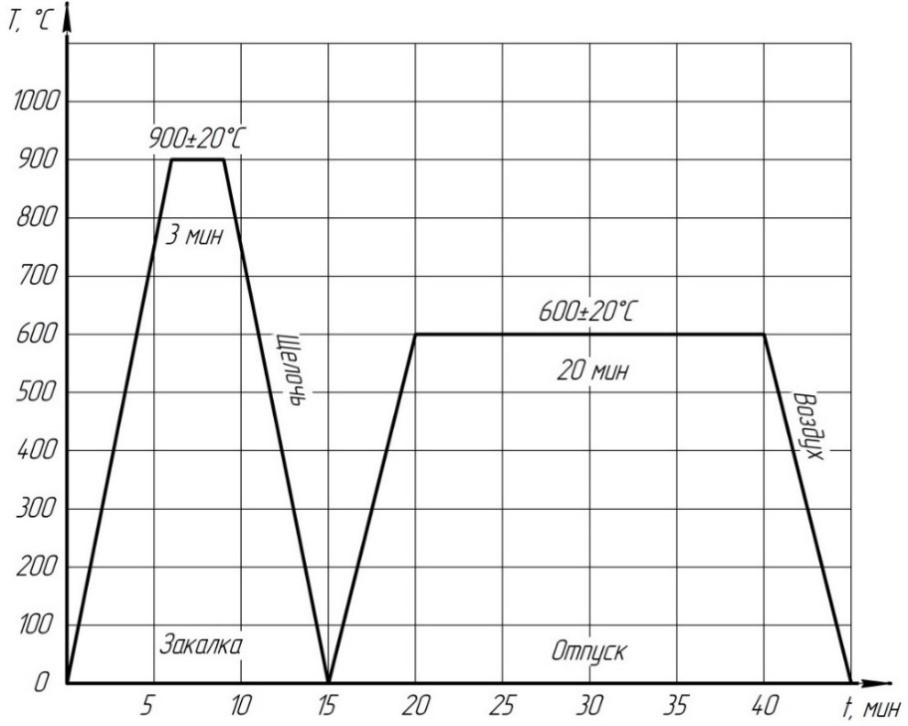
\includegraphics[width=\linewidth]{techno_termogr}
	\caption{График термической обработки}
	\label{fig:techno_termogr}
\end{figure}

\subsection{Расчет режимов механической обработки}

\paragraph{Точение}

\paragraph{Определение глубины резания $t$, мм}

Цилиндрическая поверхность диаметром $\varnothing$ 126 мм точится до $\varnothing$ 27 (операция №1, переход 7). Припуск равен t = 0.25 мм (на сторону).  Так как заданный параметр шероховатости Rz = 20 мкм (точение черновое), то точение выполняется в 1 проход, и глубина резания составляет t = 0,25 мм. 

\paragraph{Определение подачи $S$, мм/об.}

Величина подачи определяется заданным уровнем шероховатости, направлением подачи и обрабатываемым материалом. 33Х3СНМВФА.
$ s = 0.33 $ мм/об (табл.12, стр. 267 \cite{TECHNO}).

\paragraph{Скорость резания V, м/мин}

При растачивании скорость резания, рассчитывается по формуле:
$ V = \frac{C_V}{T^m t^x S_Y}$,   где

$K_V$ – поправочный коэффициент для скорости резания. $K_V = K_{MV} \cdot K_\text{ПV} \cdot K_\text{ИV}$ .

$K_\text{MV} $  – зависит от качества обрабатываемого материала.

Для 33Х3СНМВФА:	    (табл.3 стр.263 \cite{TECHNO}),

$K_\text{пv}$ – зависит от состояния поверхности ($K_\text{пv} = 0,8$ – штамповка, $K_\text{пv} = 1$ – без корки (табл.5 стр.263 \cite{TECHNO})):	$K_\text{пv} = 1,0$;

$K_\text{ИV}$ – зависит от материала инструмента (табл.6 стр.263 \cite{TECHNO}).

$K_\text{ИV} = 0,5$ – инструмент из твердого сплава ВК6, обрабатываемый материал сталь 33Х3СНМВФА.

$$K_V = 1.0 \cdot 1,0 \cdot 0,5 = 0,5$$

T, мин – стойкость резца.  Для токарной обработки принять  T = 50 мин.

Коэффициенты и показатели степени в соответствии с табл.17 \cite{TECHNO}:
– для  $s \le 0,4$   мм/об:

CV = 292, y = 0,20, x = 0,15, m = 0,20 (твердый сплав).

 $ V = \frac{292}{50^0,2 0,5^0,15 0,3_0,2} \cdot 0,5 = 94,2 $ м/мин.

\paragraph{Частота вращения шпинделя n об/мин} По установленной скорости резания определяем частоту вращения шпинделя
$ n = \frac{1000 \cdot V } { \pi \cdot D} $, где

D – диаметр обрабатываемой поверхности. Частота вращения должна быть не изменой в рамках одного перехода, поэтому рассчитывается для максимальных значений D поверхностей обрабатываемых в данном переходе.
Полученные значения округляются в соответствии с паспортными данными станка (обычно в сторону занижения). 
$ n = \frac{1000 \cdot 94,2} { 3,14 \cdot 30} =1000 $ об/мин.

Пересчитываем скорость резания при чистовом точении с учётом изменившейся частоты вращения:

$ V = \frac{n \pi D}{1000} = \frac{1000 \cdot pi \cdot 27} {1000} = 84,2$ м/мин.

\paragraph{Технологическое (основное) время  $Т_\text{ОСН}$, мин}

$Т_\text{ОСН} = \frac{L \cdot 2 } {S \cdot n}$ , где
L – расчетная длина рабочего хода режущего инструмента, т.е. путь, проходимый режущим инструментом в направлении подачи, мм.

$Т_\text{ОСН1} = \frac{77 \cdot 2 } {0.3 \cdot 1000}$ мин.

Примем $Т_\text{всп}$ = 0,5 мин, $Т_\text{пз}$= 5  мин для всех режимов.

\clearpage
\paragraph{Сила резания $P_Z$, Н. Эффективная мощность $N$, кВт}

$$P_Z = 10 C_p \cdot t^X \cdot S_Y \cdot V^n \cdot K_p$$

Коэффициенты и показатели степеней:

CP = 300, y = 0,75, x = 1, n = 0 (материал режущей части резца – ВК6) табл. 22 стр.273 \cite{TECHNO}.

	$K_{MP} = 0,75$ ; $K_\text{ФР} = 0,89$ ; $K_{\gamma P} = 1,1$ ; $K_{\lambda P} = 1,0 $  ; $K_{rp} = 1.0 $

	$$K_P = 0,75 \cdot 1,1 \cdot 0,89 \cdot 1 \cdot 1 = 0,74$$

Черновое точение $P_Z1 = 2396$  Н,

$ N = \frac{2400 \cdot 60} { 60000} = 2,4 $ кВт.

Установленные значения $P_z$ и $N$ не превышают усилия резания, допускаемого механизмом подачи станка, и эффективной мощности на шпинделе станка. Следовательно, выбранный режим осуществим.
Для обработки используется проходной упорный резец изготовленный из твердого сплава ВК6, обладающей повышенной прочностью и пригодного для изготовления режущего инструмента всех видов, в том числе для обработки обычных конструкционных материалов в условиях динамических нагрузок. В химический состав сплава входят 94\% корбида вольфрама, 6\% кобальта.

\paragraph{Сверление}

Определение глубины резания $t,$ мм.

Сверлится отверстие $\varnothing$  4 мм. При сверлении глубина резания равна $t = 0,5 \cdot D = 0,5 \cdot 4 = 2$ мм.

\paragraph{Определение подачи S, мм/об}

Величина подачи без ограничивающих факторов определяется твёрдостью материала детали и диаметром сверла. Для сверла $\varnothing$  4 мм и материала 33Х3СНМВФА выбираем подачу  s = 0,21 об/мин (табл. 25, стр. 277 \cite{TECHNO}).

\paragraph{Скорость резания V, м/мин}

Скорость резания при сверлении определяется формулой:  $ V = \frac { C_V \cdot D^q} { T_m \cdot S^Y} \cdot K_V$.

KV – поправочный коэффициент для скорости резания.

$K_V$ – поправочный коэффициент для скорости резания. $K_V = K_{MV} \cdot K_\text{tV} \cdot K_\text{ИV}$ .


$K_{MV}$  – зависит от качества обрабатываемого материала.

Для 33Х3СНМВФА: $K_{MV} = 1,1$    (табл.3 стр.263 \cite{TECHNO}),

$K_\text{ИV}$ – зависит от материала инструмента (табл.6 стр.263 \cite{TECHNO}).

$K_\text{ИV} = 1,0$ – инструмент из Р6М5, обрабатываемый материал 33Х3СНМВФА,

$K_\text{tV}$  – коэффициент, учитывающий глубину сверления (табл.31 стр.280\cite{TECHNO}).

$K_\text{tV} $=0,5 – отверстие имеет глубину 5.

$K_\text{V} = 1,0 \cdot 1,0 \cdot 0,5 = 0,55$;

T, мин – стойкость резца.  Для обработки сверлением принять  T = 25 мин (табл.30 стр.280 \cite{TECHNO}).

Коэффициенты и показатели степени в соответствии с табл.28 \cite{TECHNO}:
– для $s \le 0,2 $    мм/об:

$C_V$ = 7,0, y = 0,7, q = 0,4, m = 0,2 (быстрорежущая сталь Р6М5).

$$ V = \dfrac{ C_V \cdot D^q} {T^m \cdot S^y} \cdot K_V = \dfrac{7,0 \cdot 0,5^{0,4}}{25^{0,25} \cdot 0,21^{0,7}} \cdot 0,5 = 11,615 $$
 
\paragraph{Частота вращения шпинделя n об/мин}
По установленной скорости резания определяем частоту вращения шпинделя
 $n = \frac{1000 \cdot V}{\pi \cdot D}, n = 500 $ об/мин.

Пересчитываем скорость резания и получаем $V = 9,5$ м/мин .

\paragraph{Технологическое (основное) время  ТОСН, мин}

$ T_\text{ОСН} = \frac{L}{S\cdot n, T_\text{ОСН} = 0,9 } $ мин.

Примем $Т_\text{всп}$ = 0,5 мин,$ Т_\text{пз} $= 5  мин для всех режимов.

\paragraph{Крутящий момент Мкр, Н*м и осевая сила  P, Н.}

Данные характеристики сверления находят по формулам:
$$M_KP = 10 \cdot C_M \cdot D^q \cdot s^Y \cdot K_p ; P_0 = 10 \cdot C_p \cdot D^q \cdot s^Y \cdot K_p$$

Значения коэффициентов $C_M$  и $C_p$  и показателей степени приведены в табл. 32 \cite{TECHNO}. Коэффициенты и показатели степени в формулах крутящего момента: $C_M = 0,0345$ , q=2,0, y=0,8.

Коэффициенты и показатели степени в формулах осевой силы:
$C_p = 68$ , q=1,0, y=0,7.

Коэффициент, учитывающий фактические условия обработки, в данном случае зависит только от материала обрабатываемой заготовки и определяется выражением: $K_P = K_MP$ .

Для конструкционных сталей коэффициент $K_MP = 0,75$  (табл.10 стр.265 \cite{TECHNO}), след. $K_P$ = 0,75 .

$M_{KP} = 10 \cdot 0,0345 \cdot 6^2 \cdot 0,2^0,8 \cdot 0,75 = 2,57$ Н * м;

$P_O = 992 $ Н.

\paragraph{Мощность резания  Nр, кВт.}
Мощность резания определяют по формуле:

$$ N_p = \frac{M_kp \cdot n} { 9750} = \frac{2,57 \cdot 530} {9750} = 0,14 \text{ кВт}.$$

Допустимый крутящий момент на шпинделе станка и эффективная мощность превышает установленные расчетные значения. Следовательно, выбранный режим осуществим.

\chapter{ЭКОЛОГИЯ И ПРОМЫШЛЕННАЯ \\БЕЗОПАСНОСТЬ}
\label{cha:ch_4}

Строгое соблюдение правил безопасности и охраны труда – одно из основных условий работы. Соблюдение заранее оговоренных правил и понимание опасностей при выполнении поставленной задачи, являются главными способами борьбы с травмами и несчастными случаями на производстве. При работе с оборудованием машиностроительного производства и/или опасными веществами риск, которому подвержен работник в случае нарушения правил безопасности значительно выше, чем риск офисного работника.

В данной работе проведен анализ опасных и вредных факторов, влияющих на рабочего, при исполнении технического процесса изготовления переднего днища реактивного двигателя на твёрдом топливе (РДТТ). Процесс будет производится в цехе, в котором установлены различные виды станков. Материал заготовки – сплав СП33.

\section{Анализ опасных и вредных факторов \\ при изготовлении днища двигателя}
Технический процесс изготовления днища РДТТ включает операции и соответствующие им негативные факторы, приведенные в таблице \ref{tab:all_bad_factors}.

\begin{table}[!h]
	\begin{center}
		\caption{Опасные и вредные факторы, возникающие при изготовлении днища двигательной установки}
		\begin{tabular}{|l|p{110mm}|}
  		\hline
Тип операции & Вредные факторы \\ \hline 
Термообработка & Освещение, травмоопасность, вибрации, микроклимат. \\ \hline 
Сверление & Освещение, шум, травмоопасность. \\ \hline 
Фрезерование & Освещение, шум, вредные вещества в воздухе рабочей зоны, вибрации, ЭМИ-поля. \\ \hline 
Растачивание & Освещение, шум, вредные вещества в воздухе рабочей зоны, вибрации. \\ \hline 
Токарная & Освещение, шум, травмоопасность. \\ \hline 
		\end{tabular}
		\label{tab:all_bad_factors}
	\end{center}
\end{table}

Рассмотрев приведенные в таблице факторы, можно заключить, что на рабочего воздействует множество неблагоприятных факторов, способных привести к повышенной утомляемости и, как следствию, травме.

Также на производстве присутствует риск возникновения различных опасных факторов. Согласно ГОСТ 12.0.002-2014, опасным фактором принимается фактор производственной среды и/или трудового процесса, воздействие которого в определенных условиях на организм работающего может привести к травме, в том числе смертельной.

Список опасных факторов, которые возникают при производстве, приведен ниже.

\subsection{Электроопасность}
Основным нормативным документом, связанным с электробезопасностью, являются МПОТ (ПБ) ЭЭУ – Международные правила по охране труда и ГОСТ Р 12.1.019-2009, при эксплуатации электроустановок.
Согласно документу, следует придерживаться следующих правил обеспечения электробезопасности:
\begin{itemize}
	\item Следить за проведением рабочим, причастным к работе с электрооборудованием, инструктажей и обучений безопасным методам и приемам выполнения работ на электроустановках.
	\item Работники должны проходить обучение по оказанию первой помощи пострадавшему на производстве до допуска к самостоятельной работе;
	\item Перед началом работ на электроустановках, следует проверить исправность оборудования, а также следить за состоянием и сообщать специальному персоналу о любых неисправностях оборудования;
	\item Не допускать самовольного проведения работ в действующих электроустановках, а также снабжать персонал необходимым инвентарём для защит от электрического воздействия. 
\end{itemize}

\subsection{Пожарная опасность}
Основные требование, предъявляемые к пожарной безопасности содержатся в нормативном документе СП 4.13130.2013 «Системы противопожарной защиты. Ограничение распространения пожара на объектах защиты. Требования к объемно-планировочным и конструктивным решениям».

Согласно представленному документу, основой средств обеспечения пожарной безопасности является определение класса функциональной пожарной опасности объекта защиты, которая исходит из его целевого назначения и характеристик его основного функционального контингента. Также выбор средств зависит от степени огнестойкости здания.

Основные положения для обеспечения пожарной безопасности при изготовлении днища двигательной установки:
\begin{itemize}
	\item Снабжение производственного цеха переносными огнетушителями (ГОСТ Р 51057-2001);
	\item При работе с горючими, взрывоопасными или легковоспламенимыми веществами, следить за отсутствием по близости источников открытого огня, сварных работ, источников образования искр и т.д;
	\item Помещение должно быть снабжено системами пожаротушения, а работающий в нем персонал должен пройти инструктаж пожарной эвакуации и знать расположение ближайших аварийных выходов и путей следования к ним;
	\item соблюдение порядка хранения веществ и материалов, имеющих опасность воспламенения и тушение которых недопустимо одними и теми же средстваи, в зависимости от их химико-физических свойств.
\end{itemize}

\clearpage
\subsection{Травмоопасность}
Способность опасных производственных факторов при определен-ных обстоятельствах причинить травму работающему. Основным источником травмоопасности на предприятии и при работе в цеху обычно выступают: подвижные части механизмов, машин и узлов; подвижные элементы станков без защиты или экранов; Заготовки, необработанные поверхности, заусенцы, кромки, вылетающая при обработке стружка; падение предметов с высоты.

Основным нормативным документом, описывающим требования к безопасности персонала при работе в цеху, выступает ГОСТ 12.4.125 – 83 Система стандартов безопасности труда (ССБТ). Средства коллективной защиты работающих от воздействия механических факторов. 

\clearpage
Помимо опасных факторов, оператор также подвержен влиянию сле-дующих вредных факторов (фактор производственной среды и/или трудо-вого процесса, воздействие которого в определенных условиях на орга-низм работающего может сразу или впоследствии привести к заболеванию, в том числе смертельному, или отразиться на здоровье потомства постра-давшего, или в отдельных специфичных случаях перехода в опасный про-изводственный фактор - вызвать травму. В безопасности труда применяет-ся концепция порогового воздействия, согласно которой вредный произ-водственный фактор (исключая ионизирующие излучения) неблагоприятно воздействует на организм человека только при превышении интенсивности своего воздействия (и/или полученной дозы) выше некоторого порогового предельно допустимого значения. Последствия этого воздействия могут проявиться сразу (острое заболевание) или спустя какое-то (иногда дли-тельное - годы) время (хроническое заболевание)).

\subsection{Микроклимат}
Под микроклиматом производственных помещений понимаются ме-теорологические условия внутренней среды помещений, которые опреде-ляются действующими на организм человека сочетаниями температуры, влажности, скорости движения воздуха и теплового излучения (СанПин 2.2.4.3359-16). Микроклимат производственных помещений – это ком-плекс физических факторов, оказывающих влияние на теплообмен челове-ка и определяющих самочувствие, работоспособность, здоровье и произ-водительность труда. Поддержание микроклимата рабочего места в пре-делах гигиенических норм – важнейшая задача охраны труда.

Показатели микроклимата:
\begin{itemize}
	\item Температура воздуха;
	\item Относительная влажность воздуха;
	\item Скорость движения воздуха;
	\item Мощность теплового излучения.
\end{itemize}

Воздушная среда из всех элементов, составляющих среду обитания и деятельности человека, является важнейшей. Природный воздух представ-ляет собой сложную динамическую систему, образованную различными газами (и парами) и находящимися во взвешенном состоянии мельчайши-ми твердыми и жидкими частицами – аэрозолями.

Под загрязнением воздуха понимается прямое или косвенное введе-ние в него любого вещества в таком количестве, которое изменяет качество и состав чистого атмосферного воздуха, нанося вред людям, живой и не-живой природе.

Важнейшим газообразным веществом, определяющим качество воздуха, является водяной пар. Чем сильнее нагрет воздух, тем большее количество водяного пара он может содержать. Отношение содержащегося водяного пара к тому предельному количеству, которое может содержаться в воздухе при данной температуре, называется относительной влажностью.

Важнейшей характеристикой воздушной среды является барометрическое давление, поскольку разница барометрического давления и давления воздуха в альвеолах легких определяет величину газообмена. Барометрическое давление считается и называется нормальным на уровне моря (одна атмосфера) и экспоненциально убывает с высотой.

Помимо газового состава и барометрического давления, важнейшей характеристикой воздушной среды служит температура воздуха. В сочетании с подвижностью (скоростью) движения воздуха относительно тела человека температура воздуха определяет характер теплообмена – нагрев или охлаждение тела человека.

Жизнедеятельность человека может нормально протекать лишь при условии сохранения температурного гомеостаза организма, что достигается за счет системы терморегуляции и деятельности других функциональных систем: сердечнососудистой, выделительной, эндо­кринной и систем, обеспечивающих энергетический, водносолевой и белковый обмен.

Для сохранения постоянной температуры тела организм должен находиться в термостабильном состоянии, которое оценивается по тепловому балансу. Тепловой баланс достигается ко­ординацией процессов теплопродукции и теплоотдачи.

Микроклимат по степени влияния на тепловой баланс человека подразделяется на:
\begin{itemize}
	\item нейтральный;
	\item нагревающий;
	\item охлаждающий.
\end{itemize}

Нейтральный микроклимат – это такое сочетание его составляющих, которое при воздействии на человека в течение рабочей смены обеспечивает тепловой баланс организма, разность между величиной теплопродукции и суммарной теплоотдачей находится в пределах $\pm$ 2 Вт, доля теплоотдачи испарением влаги не превышает 30\%.

Охлаждающий микроклимат – это сочетание параметров, при котором имеет место превышение суммарной теплоотдачи в окружающую среду над величиной теплопродукции организма, приводящее к образованию общего и/или локального дефицита тепла в теле человека (> 2 Вт).

Охлаждающий микроклимат приводит к обострению язвенной болезни, радикулита, обусловливает возникновение заболеваний органов дыхания, сердечно-сосудистой системы. Охлаждение человека (как общее, так и локальное) приводит к изменению его двигательной реакции, нарушает координацию и спо­собность выполнять точные операции, вызывает тормозные процессы в коре головного мозга, что может быть причиной возникновения различ­ных форм травматизма. При локальном охлаждении кистей снижается точность выполнения рабочих операций.

Нагревающий микроклимат – сочетание его параметров, при котором имеет место изменение теплообмена человека с окружающей средой, проявляющееся в накоплении тепла в организме (> 2 Вт) и/или в увеличении доли потерь тепла испарением влаги (>30\%).

Воздействие нагревающего микроклимата вызывает нарушение состояния здоровья, снижение работоспособности и производительности труда. Нагревающий микроклимат может привести к заболеванию общего характера, которое проявляется чаще всего в виде теплового коллапса. Он возникает вследствие расширения сосудов и уменьшения давления в них крови. Обморочному состоянию предшествует головная боль, чувство слабости, головокружение, тошнота.

Тепловой удар очень опасен. Даже при раннем выявлении каждый пятый случай является смертельным. При общем тепловом застое значительно повышается температура тела, что приводит к прямому повреждению тканей, особенно центральной периной системы. Тошнота и рвота предшествуют шоковой стадии с глубокой потерей сознания, иногда сопровождающейся судорогами. Вследствие расстройства центра терморегуляции снижается потообразование. Кожа горячая, сухая, сначала имеет красный цвет, а потом приобретает серую окраску. Смертность тем выше, чем выше температура тела.

В результате солнечного удара в первую очередь нарушаются функции головного мозга из-за местного перегревания незащищенной от солнца головы. 

\begin{table}[!h]
	\begin{center}
		\caption{Параметры нормирования микроклимата, СанПиН 2.2.4.1191-03}
		\begin{tabular}{|p{21mm}|p{27mm}|p{19mm}|p{27mm}|p{33mm}|p{21mm}|}
  		\hline
Период года	& Категория работы по уровням энерготрат, Вт & Темпера- тура, °С & Температура поверхностей, °С	& Относительная влажность, \% &	Скорость движения воздуха, м/с, не более \\ 
	\hline
 Холодный & Iа (до 139) & 22-24 & 21-25  & 40-60 & 0,1 \\ 
  &Iб (140-174) &21-23 &20-24 &  &0,1 \\
  &IIа (175-232) &19-21 &18-22 &  &0,2 \\
  &IIб (233-290) &17-19 &16-20 &  &0,2 \\
  &III (более 290) &16-18 &15-19 &  &0,3 \\ \hline

 Тёплый	 & Iа (до 139) &23-25   &22-26  & 40-60 &0,1  \\ 
  &Iб (140-174) & 22-24&21-25 &  & 0,1 \\ 
  &IIа (175-232) &20-22 &19-23 &   &0,2 \\
  &IIб (233-290) &19-21 &18-22 &   &0,2 \\
  &III (более 290) &18-20 &17-21 &   &0,3 \\ \hline
		\end{tabular}
		\label{tab:eco_climat}
	\end{center}
\end{table}

Тепловое состояние человека – это функциональное состояние организма, обусловленное его теплообменом с окружающей средой, характеризующееся содержанием и распределением тепла в глубоких и поверхностных тканях организма, а также степенью напряжения механизмов терморегуляции.

Теплового состояние человека классифицируется на:
\begin{itemize}
	\item оптимальное;
	\item допустимое;
	\item предельно допустимое;
	\item недопустимое.
\end{itemize}

Разработан метод оценки теплового состояния в целях обоснования гигиенических требований к микроклимату рабочих мест, а также меры профилактики по защите работающих от возможного охлаждения и перегревания.

По степени влияния на самочувствие человека, его работоспособность микроклиматические условия подразделяются на:
\begin{itemize}
	\item оптимальные;
	\item допустимые;
	\item вредные;
	\item опасные.
\end{itemize}

Нормативные гигиенические требования к отдельным показате­лям микроклимата, их сочетаниям, разработанные на основе изучения теплообмена и теплового состояния организма человека в микро­климатических камерах и в производственных условиях, а также на основе клинических и эпидемиологических исследований, изложены в СанПиН 2.2.4.3359-16.

\paragraph{Защита работников от перегревания и переохлаждения}
Профилактика перегрева организма работника в нагревающем микроклимате включает следующие мероприятия:
\begin{itemize}
	\item нормирование верхней границы внешней термической нагрузки на допустимом уровне применительно к восьмичасовой рабочей смене;
	\item регламентация продолжительности воздействия нагревающей среды для поддержания среднесменного теплового состояния на опти­мальном или допустимом уровне;
	\item использование специальных средств коллективной и индивиду­альной защиты, уменьшающих поступление тепла извне к поверхности тела человека и обеспечивающих допустимый тепловой режим.
Защита от охлаждения осуществляется посредством:
	\item одежды, изготовленной в соответствии с требованиями государственных стандартов.
	\item использования локальных источников тепла, обеспечивающие сохранение должного уровня общего и локального теплообмена организма.
	\item регламентации продолжительности непрерывного пребывания на холоде и продолжительности пребывания в помещении с комфортными условиями. 
\end{itemize}

\paragraph{Аэроионный состав воздуха в производственных \\помещениях}

Наряду с температурой, влажностью, скоростью движения воздуха в производственных помещениях на жизнедеятельность человека оказывает влияние аэроионный состав воздуха.

В помещениях с отрицательными ионами происходит уменьшение количества микроорганизмов, снижается концентрация пыли в воздухе, нейтрализуются некоторые газы, устраняются электростатические заряды с поверхностей оборудования.

Ионизация воздуха – процесс превращения нейтральных атомов и молекул воздушной среды в электрически заряженные частицы (ионы).

В воздухе всегда имеются различные включения в виде мельчайших пылинок – аэрозолей, водяных паров и других посторонних примесей. Встречая на пути движения эти взвешенные частицы, легкие ионы соеди-няются с ними, сообщая им свой заряд. В результате таких соединений частиц образуются заряженные частицы, которые получили название тяжелых ионов. Тяжелые положительно заряженные ионы в воздухе помещений могут вызывать на коже человека угревую сыпь, прыщи, снижать эластичность кожи. Существуют сверхтяжелые ионы, которые называют аэрозолями. Они состоят из копоти, тумана, мелких дождевых капель. Такие частицы могут иметь много элементарных электрических зарядов и не нести на себе ни единого истинного газового иона.

Воздух, содержащий отрицательные аэроионы, является своеобразным экраном, отражающим излучения положительных ионов от дисплеев, телевизоров и другой оргтехники.

Естественная ионизация происходит в результате воздействия на воздушную среду космических излучений и частиц, выбрасываемых радиоактивными веществами при их распаде.

Технологическая ионизация происходит при воздействии на воздушную среду радиоактивного, рентгеновского и ультрафиолетового излучений, термоэмиссии, фотоэффекта и других ионизирующих факторов, обусловленных технологическим процессом.

Искусственная ионизация осуществляется специальными устройствами – аэроионизаторами. Физической основой большинства аэроионизаторов является коронный электрический разряд, позволяющий получать ионы нужной полярности и исключать образование вредных химических соединений (озон и окислы азота).

Нормативные уровни ионизации воздуха в производственных и общественных помещениях приведены в санитарных правилах и нормативах СанПиН 2.2.4.1294-03 “Физические факторы производственной среды. Гигиенические требования к аэроионному составу воздуха производственных и общественных помещений”. Согласно этому документу регламентируют: минимально допустимый уровень, максимально допустимый уровень, коэффициент униполярности.

Минимально допустимый и максимально допустимый уровни ионизации воздуха определяют диапазон концентраций аэроионов обеих полярностей и коэффициента униполярности во вдыхаемом воздухе, отклонение от которых создает угрозу здоровью человека. Нормативные значения уровней ионизации воздуха приведены в таблице \ref{tab:eco_ion}.

\clearpage
Измерение числа ионов в порядке текущего надзора производится один раз в квартал, а также в следующих случаях:
\begin{itemize}
	\item при аттестации рабочих мест;
	\item при организации новых рабочих мест;
	\item при внедрении новых технологических процессов, потенциально мо-гущих изменить ионный режим в зоне дыхания персонала;
	\item при оснащении рабочих мест аэроионизаторами.
\end{itemize}

\begin{table}[!h]
	\begin{center}
		\caption{Параметры нормирования микроклимата, СанПиН 2.2.4.1191-03}
		\begin{tabular}{|p{35mm}|p{27mm}|p{19mm}|p{35mm}|}
	\hline
	Нормируемые уровни & \multicolumn{2}{|c|}{Число ионов в 1 $\text{см}^3$ воздуха $\rho$ } & Коэффициент униполярности У \\
	\cline {2-3}
	& $\rho^\text{+}$ & $\rho^\text{-}$ &  \\ \hline
	Минимально допустимый & $\ge 400$ & > 600 &  $0.4 \le \text{У} \le 1.0 $ \\
	\cline {2-3}
	Максимально допустимый& \multicolumn{2}{|c|}{ <50 000 } &  \\ 
	\hline
		\end{tabular}
		\label{tab:eco_ion}
	\end{center}
\end{table}

Для современных офисных помещений задачу нормализации аэроионного состава воздуха целесообразно решать, используя ионизаторы, встраиваемые в приточные воздуховоды вентиляционных систем. Применение приточно-вытяжной вентиляции способно обеспечить относительно равномерное распределение аэронов по помещению и исключить возможность их накопления в локальных зонах. Устанавливать ионизаторы следует на незначительном расстоянии от выходной вентиляционной решетки или системы раздачи воздуха в помещение, что обусловлено значительными «потерями» аэроионов при их движении по воздуховодам (как металлическим, так и диэлектрическим) за счет нейтрализации зарядов при контакте с поверхностями.

\subsection{Вибрации}
Нормативный документ описывающий вибрации возникающие в процессе работы станков и инструментов – СН 2.2.4/2.1.8.566-96 Производственная вибрация, вибрация в помещениях жилых и общественных зданий. Санитарные нормы.

Согласно документу, вибрации классифицируются по способу передачи на человека:
\begin{itemize}
	\item общую вибрацию, передающуюся через опорные поверхности на тело сидящего или стоящего человека; 
	\item локальную вибрацию, передающуюся через руки человека.
По источнику возникновения вибраций различают:	
	\item локальную вибрацию, передающуюся человеку от ручного механизированного инструмента (с двигателями), органов ручного управления машинами и оборудованием;	
локальную вибрацию, передающуюся человеку от ручного немеханизированного инструмента (без двигателей), например, рихтовочных молотков разных моделей и обрабатываемых деталей; 
	\item общую вибрацию 1 категории - транспортную вибрацию, воздействующую на человека на рабочих местах самоходных и прицепных машин, транспортных средств при движении по местности, агрофонам и дорогам (в том числе при их строительстве). К источникам транспортной вибрации относят: тракторы сельскохозяйственные и промышленные, самоходные сельскохозяйственные машины (в том числе комбайны); автомобили грузовые (в том числе тягачи, скреперы, грейдеры, катки и т.д.); снегоочистители, самоходный горно-шахтный рельсовый транспорт;
	\item общую вибрацию 2 категории - транспортно-технологическую вибрацию, воздействующую на человека на рабочих местах машин, перемещающихся по специально подготовленным поверхностям производственных помещений, промышленных площадок, горных выработок. К источникам транспортно-технологической вибрации относят: экскаваторы (в том числе роторные), краны промышленные и строительные, машины для загрузки (завалочные) мартеновских печей в металлургическом производстве; горные комбайны, шахтные погрузочные машины, самоходные бурильные каретки; путевые машины, бетоноукладчики, напольный производственный транспорт;
	\item общую вибрацию 3 категории - технологическую вибрацию, воздействующую на человека на рабочих местах стационарных машин или передающуюся на рабочие места, не имеющие источников вибрации. К источникам технологической вибрации относят: станки металло- и деревообрабатывающие, кузнечно-прессовое оборудование, литейные машины, электрические машины, стационарные электрические установки, насосные агрегаты и вентиляторы, оборудование для бурения скважин, буровые станки, машины для животноводства, очистки и сортировки зерна (в том числе сушилки), оборудование промышленности стройматериалов (кроме бетоноукладчиков), установки химической и нефтехимической промышленности и др.
\end{itemize}

\begin{table}[!h]
	\begin{center}
		\caption{Гигиенические нормы вибрации по СН 2.2.4/2.1.8.556-96}
		\begin{tabular}{|p{30mm}|
			p{7mm}|
			p{7mm}|
			p{7mm}|
			p{7mm}|
			p{7mm}|
			p{7mm}|
			p{7mm}|
			p{7mm}|
			p{7mm}|
			p{7mm}|
			p{10mm}|
		}
	\hline
	Вид вибрации & \multicolumn{11}{|p{110mm}|}{Допустимый уровень виброскорости, дБ, в октавных полосах со среднегеометрическими частотами, Гц} \\ 
	\cline {2-12}
	& 1 & 2 & 4 & 8 & 16 & 31,5 & 63 & 125 & 250 & 500 & 1000 \\
	\hline
	Технологиче- ская & - & 108 & 99 & 93 & 92 & 92 & 92 & - & - & - & - \\
	\hline
		\end{tabular}
		\label{tab:eco_vibro}
	\end{center}
\end{table}

Общую вибрацию категории 3 по месту действия подразделяют на следующие типа:
\begin{itemize}
	\item на постоянных рабочих местах производственных помещений предприятий;
	\item на рабочих местах на складах, в столовых, бытовых, дежурных и других производственных помещений, где нет машин, генерирующих вибрацию;
	\item на рабочих местах в помещениях заводоуправления, конструкторских бюро, лабораторий, учебных пунктов, вычислительных центров, здравпунктов, конторских помещениях, рабочих комнатах и других помещениях для работников умственного труда;
\end{itemize}

Для борьбы с вибрациями, возникающими при работе станков и инструментов, подходящим вариантом будет подготовка фундамента специальной структуры и состава.

\subsection{Шум}
Основными источниками шума на рабочем месте являются:
\begin{itemize}
	\item Работающие станки и инструменты;
	\item Падающие предметы и перемещаемые заготовки;
	\item Фоновый шум со стороны окружающей застройки, транспортных магистралей и т.д.
\end{itemize}

Нормативный документ применимый к урегулированию уровня шума – СанПиН 2.2.4/2.1.8.562-96 «Шум на рабочих местах, в помещениях жилых, общественных зданий и на территории жилой застройки»
\begin{table}[!h]
	\begin{center}
		\caption{Допустимые уровни звукового давления на рабочих местах и в производственных помещениях}
		\begin{tabular}{|p{29mm}|
			p{8mm}|
			p{6mm}|
			p{6mm}|
			p{6mm}|
			p{6mm}|
			p{8mm}|
			p{8mm}|
			p{8mm}|
			p{6mm}|
				p{30mm}|
		}
	\hline
	Рабочие места & \multicolumn{9}{|p{100mm}|}{Уровни звукового давления, дБ, в октавных полосах со среднегеометрическими частотами, Гц } & Уровни звука и эквивалентные уровни звука, дБа \\
	\cline {2-10}
	& 31.5 & 63 & 125 & 250 & 500 & 1000 & 2000 & 4000 & 8000 & \\
	\hline
	В производственных помещениях и на территории предприятий & 107 & 95 & 87 & 82 & 78 & 75 & 73 & 71 & 69 & 80 \\
	\hline
		\end{tabular}
	\end{center}
\end{table}

\clearpage
Согласно таблице \ref{tab:eco_sound_pressure}, в зависимости к соответствующей трудовой деятельности следует рассматривать различные нормы допустимого звукового давления. В рассматриваемом случае данное значение – 65 дБ.
Рекомендациями для увеличения комфортабельности работы и снижению шумовой нагрузке, будут являться:
\begin{itemize}
	\item Своевременная сменный ремонт, смазка и настройка используемого оборудования;
	\item Достижение снижения уровня шума, путем акустической обработки ограждающих поверхностей помещения;
	\item Использование специальных красок и материалов, уменьшающих шум, издаваемый оборудованием.
\end{itemize}

\begin{table}[!h]
	\begin{center}
		\caption{Допустимые уровни звукового давления в зависимости от категории тяжести трудового процесса}
		\begin{tabular}{|p{35mm}|
			p{20mm}|
			p{20mm}|
			p{20mm}|
			p{20mm}|
			p{20mm}|
		}
	\hline
Категории напряженности трудового процесса & \multicolumn{5}{|p{100mm}|}{ Категории тяжести трудового процесса } \\
	\cline {2-6}
	& Легкая физическая нагрузка	 & Средняя физическая нагрузка	 & Тяжелый труд 1 степени & Тяжелый труд 2 степени	& Тяжелый труд 3 степени \\ \hline
Напряженность легкой степени  &  80  &  80  &  75  &  75  &  75 \\ \hline
Напряженность средней степени  &  70  &  70  &  65  &  65  &  65 \\ \hline
Напряженный труд 1 степени  &   60  &  60  &  -  &  -  &  - \\ \hline
Напряженный труд 2 степени  &   50  &  50  &  -  &  -  &  - \\
	\hline
		\end{tabular}
		\label{tab:eco_sound_pressure}
	\end{center}
\end{table}

\subsection{Освещение}
Действующие нормы производственного освещения описываются нормативным документом СНиП 23.05-95* Естественное и искусственное освещение.

Правильно спроектированное помещение, с необходимым количеством осветительных приборов и правильным их расположением, обеспечивают возможность нормальной производственной деятельности. При недостатках освещенности, могут возникнуть проблемы со зрением, повышенная утомляемость, нарушение центральной нервной системы, а также это может привести к травмам или нарушить общую безопасность на производстве.

В свою очередь, оказание необходимого уровня освещения позволяет обеспечить на рабочем месте необходимую производительность труда и качество выпускаемой продукции.

В рассматриваемом случае рассматривается ситуация, когда ведутся работы очень высокой точности. При этом контрастность объекта с фоном средняя, как и характеристика фона. В связи с этим при системе комбинированного освещения значение нормированной минимальной освещенности составляет Еmin=300 лк.

\section{Расчёт искусственного освещения \\рабочего помещения}
Поскольку одним из основных недостатков концентрических ПОУ являются высокие требования к точности изготовления, необходимо создать достаточно благоприятные условия для изготовления оных. Важнейшим фактором в этом случае будет являться освещение цеха, расчёт которого и будет произведён в этом разделе.

Рассчитать систему искусственного освещения для создания на рабочих местах нормируемой освещённости в цехе для механической обработки размерами: длина А =50 м, ширина В = 20 м, высоте Н = 9 м. В цехе выполняются работы высокой точности (наименьшие размеры объектов различения 0,15 мм), фон - темный, контраст - средний, выделение пыли -  значительное. 

Выбираем дуговые ртутные люминесцентные лампы (ДРЛ), рекомендуемые для высоких цехов при работе с поверхностями без выраженной цветности (металл); выбираем общее освещение, так как до всей площади помещения выполняются однотипные работы; для ламп ДРЛ рекомендуются специальные светильники СЗ4ДРЛ прямого свете с зеркальной отражающей поверхностью, так как помещение высокое, а отражающая способность стен и потолка малая. 

Размещаем светильники равномерно четырьмя рядами (рисунок \ref{fig:plant_light_scheme}). Расстояние между рядами светильников L определяем на условия:

$$ \frac{L}{3} + L + L + L + \frac{L}{3} = B \Rightarrow L = \frac{20 \cdot 3}{11}=5.45 м; \frac{L}{3} = 1.81 м $$

\begin{figure}[!h]
\begin{center}
	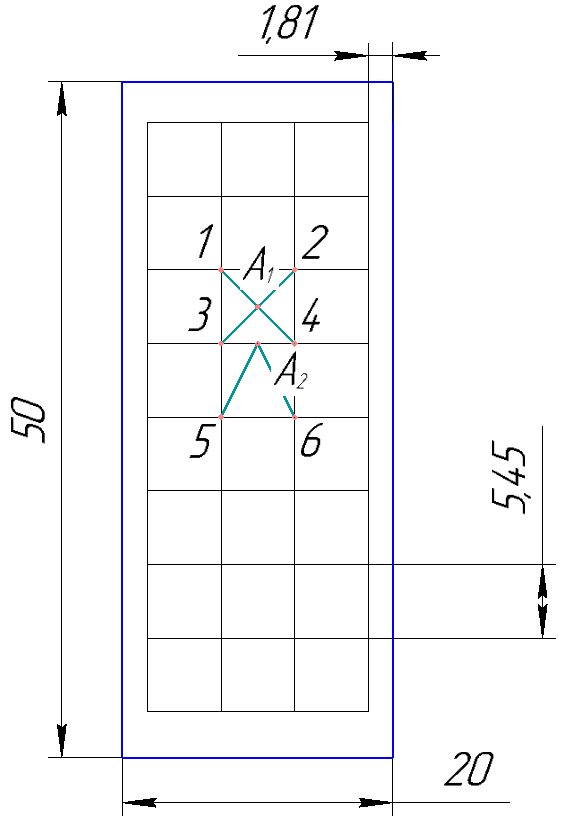
\includegraphics[height=10cm]{plant_light_scheme}
	\caption{Схема размещения светильников}
	\label{fig:plant_light_scheme}
\end{center}
\end{figure}

Количество светильников в ряду:
$$ \frac{A}{L} = \frac{50}{5.45} = 9 $$

Общее число светильников:
$$ N = 4 \cdot 9 = 36 $$

Высоту повеса светильников над уровнем пола определяем из условия их наиболее выгодного светотехнического расположения:
$$ h =L \cdot \lambda=5,45 $$

Значение h оказалось больше минимально допустимой высоты подвеса светильников над полом, следовательно, выполнено требование норм по ограничению ослепленности осветительной установкой. 

В соответствии с характером работ, системой освещения и типом источника света минимальная нормируемая освещённость Е= 300 лк, коэффициент запасе k = 1,8.

Проводим расчет по точечному методу, рекомендуемому для больших цехов с малой долей отражённого света, для контрольных точек А1 и А2 (рисунок \ref{fig:plant_light_scheme}). Ниже приводится порядок этого расчета, а его результаты сведены в таблице \ref{tab:ecolog_results}:
\begin{enumerate}[1.]
	\item Тангенс угла падения светового луча от ближайших светильников tg $\alpha=\frac{d}{h}$, где d - проекция расстоянии от контрольной точки до светильника на горизонтальную плоскость (определяется по чертежу), h - высота подвеса светильника, h= 5,45 м;
	\item Угол $\alpha$ и $\cos \alpha$ определяем по найденному значению $\tg \alpha$;
	\item Силу света $J_\alpha$ условной рампы в 1000 лм для выбранного типа светильника и угла $\alpha$ определяем из методического пособия  \cite{ECO};
	\item Освещенность от i-го светильника в расчетных точках определяем по формуле $E_{Аi}=\frac{J_\alpha \cdot \cos^3 \alpha \cdot \mu}{k \cdot h^3 } $ где $\mu$ - коэффициент, учитывающий действие удаленных светильников ($\mu$= 1,15);
	\item Суммарная освещенность в каждой из контрольных точек, создаваемая ближайшими светильниками: $E_A = \sum_{i=1}^n E_{Ai} $;
	\item Расчётный световой поток (в люменах), который должен быть создан каждой лампой для получения в расчётной точке нормируемой освещённости $E_\text{н}$: F=1000 $\frac{E_H}{E_A}$ ;
	\item Подбираем в соответствии с полученным значением F лампу требуемой мощности $P_A$. При выборе мощности лампы следует принимать значение ближайшего большого светового потока;
	\item Суммарная мощность имеющейся в производственном помещении осветительной установки: $P_\Sigma = P_A \cdot N $=25200 Вт.
\end{enumerate}

\begin{table}[!h]
	\begin{center}
		\caption{Результаты проверки на контрольных точках}
		\begin{tabular}{|p{22mm}|
			p{25mm}|
			p{8mm}|
			p{12mm}|
			p{10mm}|
			p{10mm}|
			p{10mm}|
			p{10mm}|
			p{11mm}|
			p{8mm}|
		}
	\hline
	Контроль- ная точка  & Светильник № & d,м & $\tg \alpha$ & $\alpha$,° & $J_\alpha$, кв & $E_{Ai}$, лк & $E_A$, лк & F, лм & $P_A$, Вт  \\
	\hline
 	A1 & 1 & 3,86 & 0,708 & 35,3&  305 &2,55 & 10,2 & 29412 & 700 \\
	\cline {2-8}
& 2 & 3,86 & 0,708 & 35,3 & 305 & 2,55 & 10,2 & & \\ 
	\cline {2-8}
& 3 & 3,86 & 0,708 & 35,3 & 305 & 2,55 & 10,2 & & \\
	\cline {2-8}
& 4 & 3,86 & 0,708 & 35,3 & 305 & 2,55 & 10,2 & & \\
	\hline
 	A2 & 3 & 2,73 & 0,5 & 27 &  305 & 4,2 & 10,1 & 29703  & 700 \\
	\cline {2-8}
& 4 & 2,73 & 0,5 & 27 & 305 & 4,2 & 10,1 & & \\
	\cline {2-8}
& 1 & 6,1 & 1,12 & 50 & 305 & 0,44 & 10,1 & & \\
	\cline {2-8}
& 2 & 6,1 & 1,12 & 50 & 305 & 0,44 & 10,1 & & \\
	\cline {2-8}
& 5 & 6,1 & 1,12 & 50 & 305 & 0,44 & 10,1 & & \\
	\cline {2-8}
& 6 & 6,1 & 1,12 & 50 & 305 & 0,44 & 10,1 & & \\
	\hline
		\end{tabular}
		\label{tab:ecolog_results}
	\end{center}
\end{table}

\section{Экологическая экспертиза проекта}
\paragraph{Утилизация и переработка металлической стружки}

Высокопроизводительные металлообрабатывающие станки, использующие скоростную резку, нуждаются в больших объемах охлаждающей жидкости и производят огромное количество металлической пыли и стружки. Использование таких станков приводит к интенсивному использованию металла, ресурсы которого неумолимо сокращаются. Это приводит к дефициту и подорожанью этого сырья. Учитывая, что запасы руды небезграничны, а легкодоступный металлический лом практически исчерпан, возникает вопрос поиска новых возможностей пополнения сырья для возобновления запасов металла.

Одним из таких способов является сбор и последующая переработка металлической стружки, которая возникает в процессе обработки различных деталей на металлообрабатывающих станках.

Металлическая стружка является продуктом обработки различных металлических деталей с помощью разного рода технологического оборудования.

В процессе работы с деталями на заводах и предприятиях может образовываться большое количество стружки, общий вес которой может составлять до 10\% от массы обрабатываемых деталей. Это очень большое количество отходов, которые могут успешно применяться в процессе повторной переработки для получения новых металлических заготовок.

Сбор и транспортировка стружки осложняется тем, что эти отходы имеют небольшую плотность. Это приводит к тому, что контейнер для сбора металлической стружки быстро наполняется, а для перевозки отходов на перерабатывающее предприятие требуется большое количество транспортных средств или много дополнительных рейсов.

Проблемы возникают и в процессе переработки необработанной стружки. Если переплавка производится непрессованной стружки, то возникают существенные потери металла вследствие большого угара этого вторсырья и окисления легирующих элементов, содержащихся в стальной стружке. Это в свою очередь приводит к снижению качества получаемой стали.

Чтобы исключить перечисленные проблемы, на предприятиях используют специальные механизированные системы для сбора, хранения и транспортировке стружки и подготовки ее к последующей утилизации и переработке.

Переработка производственных отходов в виде металлической стружки подразумевает под собой повторную переплавку этого вторсырья с целью получения нового металла.


\paragraph{Утилизация стружки чёрных металлов}

Большой процент металлической стружки приходится на черные металлы (сталь, чугун). Прием стружки металлической черных металлов производится в соответствии с ГОСТом 2787-75, который определяет классы стружки и требования к ее состоянию.

К основным особенностям относится то, что стружка не должна иметь ржавчину, за исключением небольшого налета, также не должно быть следов воздействия отжига, кислоты. Ограничено и наличие маслянистых отложений на металлической стружке.

Если стружка соответствует описным в ГОСТе параметрам, она отправляется на повторную переплавку.

\paragraph{Утилизация стружки цветных металлов}

Переработка металлической стружки цветных металлов имеет свои особенности, которые связаны с выполнением определенных условий по чистоте стружки от различных примесей. Отбор и процесс переработки цветной стружки регламентируется ГОСТом 28053-89. В нем описаны рекомендации по выбору и использованию методик для отбора стружки.
На крупных перерабатывающих предприятиях используют несколько методов для распределения стружки по категориям:
\begin{itemize}
	\item визуальный осмотр;
	\item учет магнитных свойств материала;
	\item химический анализ состава.
\end{itemize}
После соответствующего отбора стружка отправляется на переплавку, в процессе которой могут отбираться пробы для проведения спектрального анализа чистоты получаемого металла.

\paragraph{Оборудование для утилизации}

Процесс утилизации металлической стружки упрощается за счет использования специальных механизированных комплексов, которые позволяют подготовить вторсырье для последующей переплавки. Эти комплексы включают в свой состав различное функциональное оборудование.

\paragraph{Дробилки}

Эти установки используются для измельчения металлических отходов с целью того, чтобы на выходе была мелкая металлическая стружка, которая впоследствии будет брикетирована.

Дробилки позволяют измельчать стружку за счет ее резанья, трения друг о друга. Такие установки подходят для дробления как отходов черных материалов, так и цветных.

\paragraph{Центрифуги}

Установки этого типа применяются для очистки и осушения дробленной металлической стружки.

С помощью этих устройств можно выделить из стружки остатки масла и различных эмульсий и произвести сушку металла перед его брикетированием.

\paragraph{Прессы}

Это установки, с помощью которых осуществляется прессование металлической стружки.

После обработки на прессе получают компактные брикеты с высокой плотностью, из которых получают высококачественный переплавленный металл.

\chapter{ОРГАНИЗАЦИОННО-ЭКОНОМИЧЕСКАЯ ЧАСТЬ}
\label{cha:ch_5}


\backmatter %% Здесь заканчивается нумерованная часть документа и начинаются ссылки и
            %% заключение

\Conclusion % заключение к отчёту

Текст заключения


\nocite{*}
\bibliographystyle{gost780u}
\bibliography{0-main}


\appendix   % Тут идут приложения
\chapter{ПРОЕКТИРОВАНИЕ ДВИГАТЕЛЬНОЙ \\ УСТАНОВКИ}
ДУ образца представляет собой стартовый РДТТ на смесевом топливе.

Определение конструктивных параметров РДТТ будет осуществляться по результатам варьирования давления внутри камеры сгорания. Назначим следующий диапазон варьирования:
\[ \text{от 5 МПа до 25 Мпа, с шагом 1 МПа.}
\]

\section{Исходные данные}
\begin{table}[!h]
	\begin{center}
		\begin{tabular}{l l l}
Калибр:				 &  & $D_\text{н}$=125 мм \\ 
Полный импульс:		 &	& $J_\text{p}$= 3300 Н$\cdot$с \\ 
Материал корпуса ДУ: &	& сплав СП-33 \\
Время работы ДУ:	 &	& 3.5 с \\ 
%					 &	$\rho_\text{м}$=7830  кг/м^3  \\ 
%					 &	$\sigma_\text{вр}$=1650 Мпа	 \\ 
%					 &	$\sigma_\text{02}$=1350 Мпа	 \\ 
		\end{tabular}
		\label{tab:hellfire_stats}
	\end{center}
\end{table}



\end{document}
